\documentclass[12pt, a4paper,oneside]{report}
\usepackage{titlesec}
\usepackage[utf8]{inputenc}
\usepackage[T1]{fontenc}
\usepackage{textcomp}
\usepackage{framed}
\usepackage{pbox}
\usepackage{caption}
\usepackage[nottoc,numbib]{tocbibind}
\usepackage[pdftex]{graphicx}
\usepackage[toc]{glossaries}
\usepackage{tabularx}
\usepackage{colortbl}
\usepackage{hhline}
\usepackage{amssymb, amsmath}
\usepackage{blkarray}
\usepackage[colorlinks,
pdfstartview = FitH,
linkcolor = black,
plainpages = false,
hypertexnames = false,
citecolor = black]{hyperref}
\usepackage{setspace}
\setstretch{1.25}
\usepackage[left=3.5cm,right=3.5cm,top=2cm,bottom=2cm]{geometry}
\graphicspath{{./pics/}}
\usepackage[printonlyused]{acronym}
\usepackage{todonotes}
\usepackage{subcaption}
\usepackage{float}
\usepackage{pifont}
\newcommand{\cmark}{\ding{51}}%
\newcommand{\xmark}{\ding{55}}%
\usepackage{multirow}
\usepackage{pdflscape}
\usepackage{eurosym}
\usepackage{tocbibind}
\usepackage[english]{babel}
\usepackage[utf8]{inputenc}
\usepackage{multirow}
\usepackage{subcaption}
\usepackage[section]{placeins}
\usepackage{lscape}
\usepackage{adjustbox}
\usepackage{graphicx}
\usepackage{amsmath}
\usepackage{algorithm}
\usepackage{booktabs}
\usepackage{tabularx}
\usepackage{placeins}

\setcounter{secnumdepth}{5}
\usepackage{parskip}


\begin{document}

\begin{titlepage}
	Universität Passau\newline
	Fakultät für Informatik und Mathematik
	\vspace{2.5cm}
    \begin{center}
    \LARGE\textbf{{Classification  Of Visualization  In Scientific Literature}}\\
   
    \normalsize

    \vspace{2.5cm}
    \end{center}

 \normalsize{
 	Masterarbeit zur Erlangung des akademischen Grades\newline
 	Master of Science (M.Sc.)\newline
 	\ \\
 	Lehrstuhl für Intelligent Systems und Lehrstuhl für Data Science \newline
 	der Fakultät für Informatik und Mathematik\newline
 	der Universität Passau\newline
 	
 
    \begin{tabular}{ll}
    	Name: & Arnold Azeem \\
    	Matrikelnummer: & 79176 \\
    	Fachbereich: & Informatik\\
    	Studiengang: & Master Informatik\\
	Erstprüfer: & Prof. Dr. Christin Siefert \\
	Zweitprüfer: & Prof. Dr. Michael Granitzer\\
	Date: &     \today
    \end{tabular}\\
    }



\newpage
\begin{abstract}
Distinct visualisation techniques are used in scientific research publications to summarise large amount of data and also represent a variety of data. These visualisations help to communicate complex information and support the arguments being presented in the publication in a way that is easy to understand and follow.
These figures tend to reveal trends, patterns or relations that might have otherwise been difficult to grasp using only text. 
It is therefore relevant that we extract the data from these visualisations since the extracted data can be used for validating the publication or presenting the data in another form for a different audience. In this context, classifying these visualisations is the initial step since, there is a variety of visualisations and each one is processed in a specific way. It is only after classification that extraction of raw data from these visualisations can be acquired for other tasks. This thesis presents an approach whereby real world data is used to create four types of plots (scatter plots, bar charts, line charts, and box-plots) and random plots also of the same kind from the Internet are added together and used to train and evaluate a CovNet model to be able to classify these plots. 
\end{abstract}

\renewcommand{\abstractname}{Acknowledgements}

\end{titlepage}
\setcounter{tocdepth}{10}

\clearpage
\tableofcontents


% \begin{acronym}

% \acro{XML} {Extensible Markup Language}s

% \end{acronym}

\listoffigures
\listoftables

\titleformat{\chapter}{\LARGE\bfseries}{\thechapter}{1em}{}

\newpage


\newpage
\chapter{Introduction}
``The human brain processes images 60,000 times faster than text, and 90 percent of information transmitted to the brain is visual'' \cite{humaneye}. As human beings, we have been communicating amongst each other for a much longer period of time than we have been using written words. Our brain is therefore inclined more to processing visual data faster than text.

Due to this fact, most scientist, therefore, exploit the brain's ability to capture visualized content faster by representing their research findings using chart images and then embedding these images in their publications. Since data is ever growing and more visualizations are being used, there is a growing need for these graphs to be analyzed faster and automatically. Identifying or classifying these charts serves as a foundation for further analysis of the content of these charts.  

The aim of this thesis is to develop a reliable dataset consisting of chart images which will enable us to train a model capable of classifying chart images accurately as an initial step towards decoding the content by a machine. The structure of this thesis comprises of chart creation, image processing, and machine learning techniques.

The initial section in this chapter gives an overview of chart image classification and the complications and difficulties faced in chart image classification. In the other sections of this chapter the research motivation, objectives, contributions and an outline of the proposed framework in this thesis is presented. Finally, the structure of the rest of this thesis is illustrated in Section 1.6.

\section{Overview} 
A basic description of a chart is a graphical representation of data, where the data is represented by some type of symbols. These symbols could be rectangles in the case of histograms or bar charts,  slices that make a circle in the case of a pie chart, and dots, stars, diamonds and an asterisk in the case of a scatter plot. Charts are often used to visualize complex data for easy understanding, interpretation, and to find patterns and trends in data. Charts can usually be read more quickly than the raw data visualized, they are used in almost every field especially in science, marketing, and maths. Charts are mostly created with the help of a computer but can also be created by hand. There are a variety of charts and therefore, to present your data in the right way, the right type of chart must be employed. For example bar charts are best used when comparing data, line charts work better when we want to find trends in data and scatter plots are used when we want to find relationships in data. Figure \ref{fig:chartse} which was inspired by a diagram from \cite{chartselection} shows which charts we should choose depending on what task we would like to describe. For example, if we want to show a relationship between two variables in some data, a scatter plot is the best option, as seen below.\\

\begin{figure}[!htb]
	\centering
	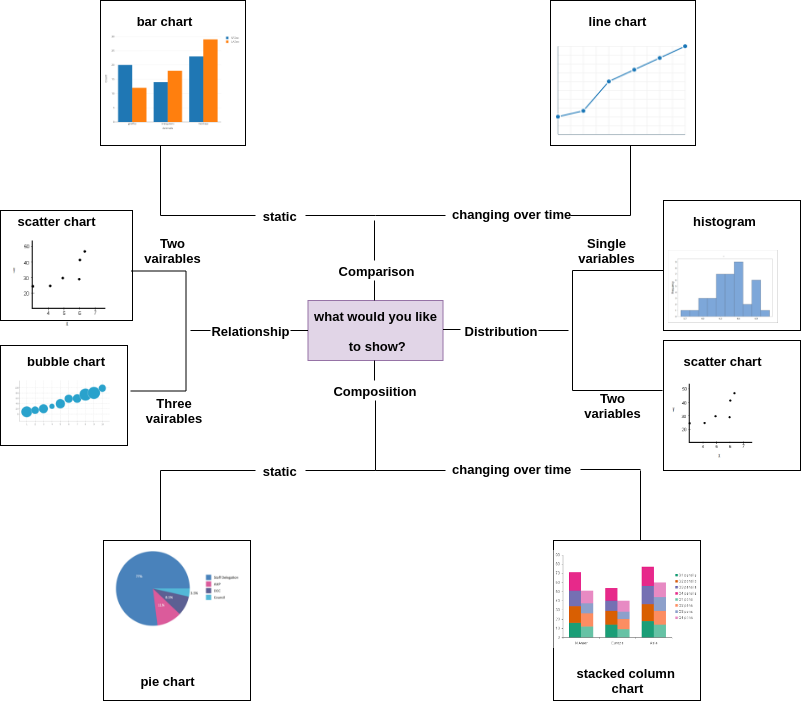
\includegraphics [scale=0.5] {chart}
	\captionof{figure}{How to Seletect the approapriate chart for visualizing your data }
	\label{fig:chartse}
\end{figure}

Charts usually appear in different forms, nonetheless, there are some features that are mostly present in every chart. Charts are mostly graphical with a little bit of text used to annotate the data. One important use of text, visible in most charts is to give the chart a title. The title describes what the graphic represents and is usually situated above the main graphical part. Text is used less because the brain processes visual information sixty thousand faster \cite{humaneye} as mentioned earlier. Most graphs have one line at the side and another usually at the bottom. These lines if used are called axes of the graph. The one at the bottom is called the x-axis, and the other line is the y-axis. Each graph usually indicates numerical or periodic sequence shown by periodic graduations. There are also texts usually outside or beside the axis describing the measurements.
Some charts include what we call a legend, the legend is usually present in situations where there are multiple variables to be described. Figure \ref{fig:boxy} shows a typical chart that has the features mentioned above. The legend showing the two variables female and male represented in the chart, the label on the left side annotating the cholesterol levels with the different measurements of the cholesterol shown on the y-axis, and to the bottom categorical measurements shown on the x-axis. Finally, the title that is the text describing the whole chart is mostly shown at the top of the visual graph. 

\begin{figure}[!htb]
	\centering
	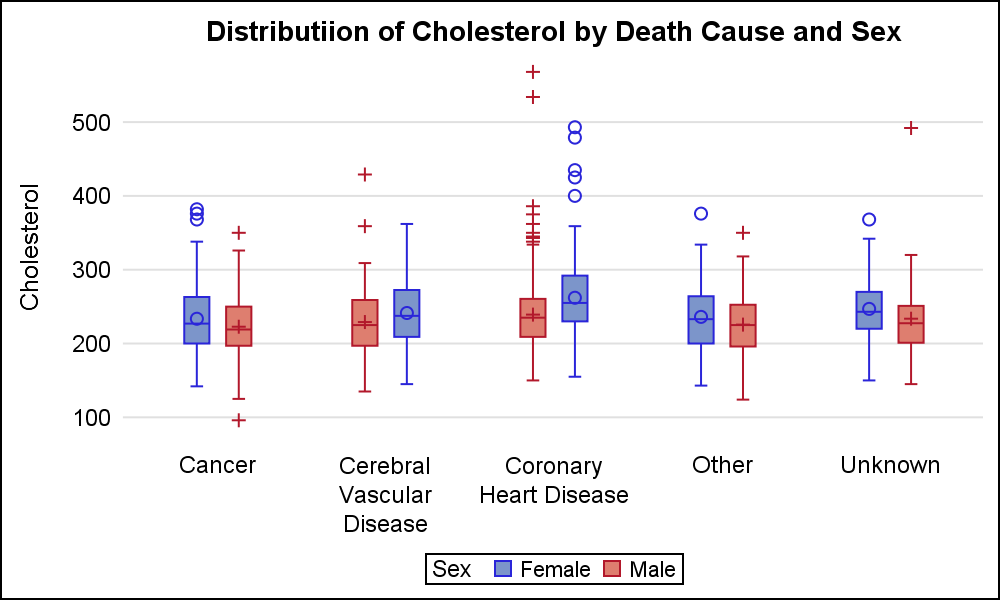
\includegraphics [scale=1.0] {box_color.png}
	\captionof{figure}{A box plot with a legend, x-axis, and y-axis from \cite{boxy} }
	\label{fig:boxy}
\end{figure}

Despite most features being present in most charts, there are some charts that are totally different from the rest. For example, a pie chart does not have an x-axis or y-axis, also the designers of a particular chart have a choice of visual encoding and styling, this results in a wide variety of charts, even in charts of the same type. To be able to identify the different types of charts accurately will mean, considering all the wide range of the different visual encodings and styles of these charts.

\section{Motivation}
The examples described in the introductory section have shown that chart images are very relevant for visualizing data and there is a need to classify chart images as a basis for further analysis of the charts. Charts contain a wealth of information that other researchers will like to extract and interpret because:
\begin{itemize}
	\item The information when extracted can be used by another researcher to validate the authenticity of the experiment done and the results obtained.
	
	\item The information of one type of chart can be decoded and presented in another form to a different audience.
	
	\item Comparing two chart is more effective when we have access to the raw data.
\end{itemize} 

Even though the identification, analysis, and interpretation of chart data can easily be done by a human being, machines, on the other hand, find it difficult to decode them due to the variations in their appearance and their variable structure~\cite{liu2015chart}. There is a growing need in many fields for machines to be able to perform tasks that human beings are easily doing with regards to chart analysis~\cite{amara2017convolutional}. 

In spite of this growing interest, there have been little groundbreaking results achieved due to the complexity of the problem~\cite{liu2015chart}. Previous research on chart classification exploited the structural content of charts for classification. For example, Manollis Savva, et al.  ~\cite{savva2011revision} proposed a model to classify charts
using extracted low-level features (small rectangular image regions)and textual features. After extracting the features, a  Support Vector Machines (SVMs) classifier is used for the classification step. This method was limited since most charts contain the same types of low-level features like axes, grid lines, and legends. In V. Shiv Naga Prasad's work~ \cite{prasad2007classifying} classification was based on using features based on the shape and spatial relationships of their primitives. This work was limited due to the inconstancy in which data in most charts can be depicted. In the paper of Alex Krizhevsky et al.~\cite{krizhevsky2012imagenet} a deep CovNet (this abbreviation stands for Convolutional Neural Networks and will be used a lot through this work) which combines both feature extraction and classification was used and this technique achieved good results. However, the dataset size of 3377 chart images of 11 classes is a bit limited due to the complexity of the problem. 

These, and more problems addressed in Chapter 2 motivated us to find a more efficient solution, in this report, we therefore, present our attempt at a probable solution.

\section{Objective}
The aim of this thesis is to develop algorithms using image processing and machine learning methods for the purpose of chart image classification. Different approaches will be considered in other to choose the most favorable one.\\
The goal of this thesis is to try to identify or recognise chart images with the highest accuracy. To achieve this goal we have to answer the question: \begin{quote} How Well Can We Classify the Four Different Types of Plots (Line-Charts, Bar-Charts, Scatter-plots, and Box-plots) in Scientific Literature? \end{quote} 
To answer this question, the following objectives are set.

\begin{itemize}\itemsep3pt
	\item obtain raw data gathered from real world occurrences.
	\item create a dataset of chart images with the collected data. Using  different plotting programs (Python, Matlab, R, and Java) and different libraries supported by these plotting programs.
	\item train and evaluate a machine learning model that can recognise unseen charts with high accuracy. The four classes of plots are box plots, line charts, scatter plots and, bar-charts.
\end{itemize}

\section{Research Significance and Contribution}
Figure \ref{fig:vis} shows the significance of this work and what it will lead to. This thesis focuses mainly on four chart images. These plots are scatter plots, bar charts, line charts and box plots. The first three were selected because, they are the most popular image charts and box-plots because it shows skewness and unusual observations in a dataset, and this information is especially relevant when dealing with large data, which is mostly the case in machine learning. The first part of Figure \ref{fig:vis} involves, obtaining  the four different types of plots mentioned earlier, after which we then label our plots and train a neural network model to classify with high accuracy any of the four plots if shown to our model, then finally the raw data can be extracted from the detected plot using other processes and techniques. The focus of this thesis however, is shown in the figure with red dotted lines, which entails, gathering a dataset of chart images, labeling them, training a model that can classify the plots. \\

\begin{figure}[!htb]
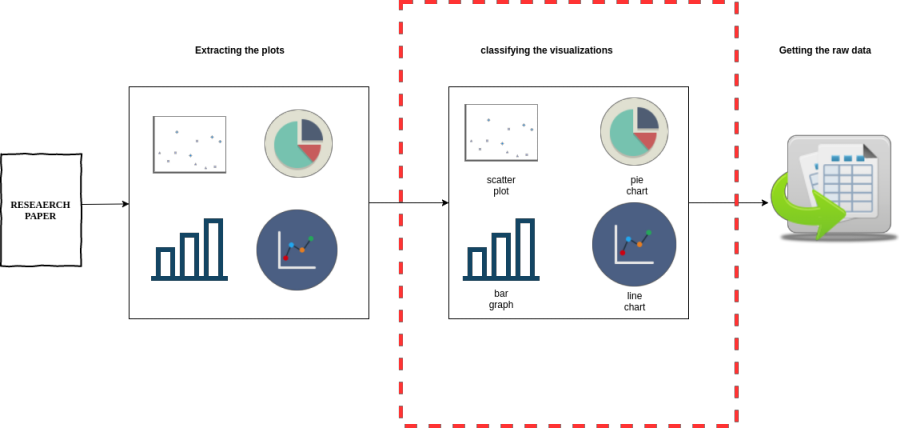
\includegraphics [scale=0.48] {vision}
\captionof{figure}{Overview of process to obtain raw 
	data from scientific papers. The red outline indicates the work in this 
	thesis.}
\label{fig:vis}
\end{figure}


\chapter{Background and Related Work}
\section{Overview}
In this chapter, the literature on the classification of chart images is presented and explored. Old techniques that were previously used and how they evolved are discussed. Section 3.2 introduces the two main categories of image classification, while in 3.3 and 3.4 the two categories are discussed in detail, also, CovNets which are inspired by the cat’s visual cortex and have performed really well in the field of image processing is talked about in detail. Lastly, Section 3.5 presents the important approaches and techniques employed by other researchers for chart image classification.

\section{Background}
Classification involving charts images has been a topic of huge interest in recent times. This is due to the fact that, most scientific publications if not all, are embedded with these charts as a way of conveying complex research findings in more visualizable and easy to understand format. As a result of this popularity, chart images have gained, different techniques have over time been used for classifying these chart images, these methods have over the past few years evolved. The techniques in recent years have been inspired by the field of image processing which employs raster to vector conversion and layout analysis of the images amongst others. These techniques can be put into two main categories, Model-Based Approaches and Machine Learning Based Approaches ~\cite{amara2017convolutional}. 

In the next section, the approach used in this thesis, and the works that inspired us to choose these techniques are explained in details.

\section{Model Based Approaches}
The following is written with inspiration from Boyle et al. work~\cite{boyle2007advances}. Numerous chart images even of the same type, are different in sense of their context structure. This is as a result of the variability of the positions of the context structure of a chart. There is exists no real standard for all charts to follow, content like legends, axes, grids etc., have no fixed position and sometimes are not even present in some charts. As a result of this non-standardization of charts, classifying becomes a difficult task. Initially, chart classification exploited the structure of charts, this method is generally called model-based. The model-based approach is divided into two steps. Firstly, a number of predefined object classes are created with abstract models and then an image is matched with the created model. For example, a model for a 2D/3D pie chart consists of line segments (radii and circular/elliptical arcs), and these line segments are used to create the model, however, just using these line segments won't be enough, so some constraints are introduced into the model, example of constraints of a pie chart include; the center of the pie chart is where all radii meet; all 2D pie charts have radii of equal length; arcs mainly form parts of the same 2D pie chart circle, or if its a 3D then the arcs form part of the ellipse. After this, a goodness-of-fit is introduced to help measure the discrepancy between the image and the conditions for the model. For example, a goodness-of-fit of a pie chart is as follows: the difference in length of radii, the difference in how the arcs are curved, the distance between a center of a circle and that of a radii. When a chart is presented for classification, the edges are detected, thinned, linked, vectorized, extracted and compared to the various edge models created and the best match is selected. After this, the good-to-fit criteria is used to measure the difference between the edges of the model and the image. Finally, a voting is performed base on the value of the good-to-fit results. The model-based approach has some drawbacks though. The main drawback is that human intervention is needed to develop the various models. This could be a cumbersome and time-consuming procedure, due to the limitation of this approach a machine learning approach was introduced to handle some of the limitations of this approach.


\section{Machine Learning Based Approaches}
This method was developed in recent times, and most works in the area of image analysis and processing employ this approach. This method involves using handcrafted features extracted from the charts for the classification task. In Zhou and Tan's ~\cite{zhou2000bar} work, features like a legend, x-y-axis labels, chart title, and values of the bar of a bar-chart were extracted for purposes of classifying a bar-chart. In Shao and  Futrelle's~\cite{shao2005recognition} work, graphical elements of the charts like colors, tick marks on an axis and data point markers are the handcrafted feature used for classification. Another instance where handcrafted features were used was in Inokuchi et al. work~\cite{inokuchi2000apriori}. In this work, regular appearing substructures of a chart are extracted and used as features for classification. After the feature acquisition step, the obtained features are then represented in vector form for the classification step. The features are stored in a matrix vector-like structure. Algorithm~\ref{alg:1} shows an example of the structure in which the features are stored. This structure has multiple columns containing the features and one column indicating the target or label of the chart. This vector-like structure is then fed as input into a machine learning technique for the model training step. In Karthikeyani and Nagarajan's paper~\cite{karthikeyani2012machine} after the features were obtained SVM Classification \footnote{http://www.statsoft.com/Textbook/Support-Vector-Machines}, MLP Classification
\footnote{http://www.iro.umontreal.ca/~bengioy/ift6266/H12/html/mlp\_en.html}, and  KNN Classification\footnote{
https://kevinzakka.github.io/2016/07/13/k-nearest-neighbor/} were used to create a function that maps the set of features to a predefined label. This technique achieves good results but, the drawback is that there is an over-reliance on handcrafted features. This drawback makes it difficult when a large amount of data consisting of a variable context structure is involved, and this situation is evident in most cases. Recently, however CovNets \footnote{https://deeplearning4j.org/convolutionalnetwork}, a machine learning technique which removes the drawback of using handcrafted features by learning important features anywhere in the image automatically. CovNets performance on image classification keeps on improving and in recent times, results are being compared to human performance levels. CovNets were used in this work, in the next section they will be explained in details.

\section{Convolutional Neural Network}

\subsection{Artificial Neural Networks}
This section is inspired by a book called the nature code~\cite{naturecode}. Artificial neural network a very important tool in machine learning was developed with inspiration from the inner workings of the human brain to solve certain kinds of problems. There are certain kinds of problems that are easy for a computer to solve but rather difficult for human beings. There are also on the other hand problems that are easier for human beings to solve but difficult for computers. Show me a picture of a cow today and tomorrow I can pick a different picture of a cow from a group of pictures of animals. But when its time for a machine to perform the same task it becomes more complicated. There has been a lot of research into finding solutions for tasks such as the one mentioned above.

Artificial neural networks have been found to perform really well in tasks difficult for computers but easier for human beings. One property that makes neural networks standout is their ability to learn. A neural network is a system that can change its inner workings based on the information flowing through it. This is possible because it can adjust what we call its weights.
Figure~\ref{fig:neural} is a representation of a typical neural network. In the diagram, each line indicates a path of flow of information. These lines are represented by numbers(weights). In an event where there is a bad output, these weights are adjusted by the system in other to improve subsequent results. This ability to learn and make an adjustment in other to improve its results is what makes neural networks special in machine learning. Neural networks perform really well in fields like pattern recognition, anomaly detection, signal processing, and, image classification.

\begin{figure}[!htbp]
	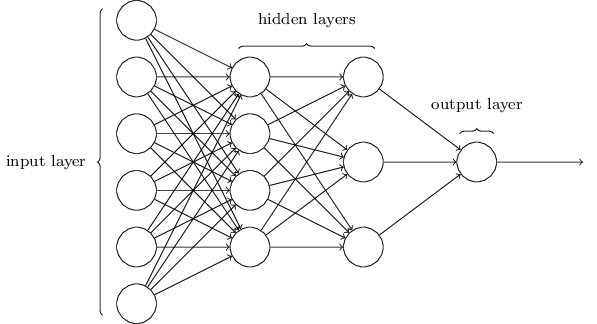
\includegraphics [scale=0.7] {neural.png}
	\captionof{figure}{How a neural network look like}
	\label{fig:neural}
\end{figure}

\subsection{Convolutional Neural Network}
CovNets are a category of neural networks that have archived state of the art results in the area of image classification and analysis. Neural networks have fallen out of use due to the fact that information flows from input to output in one direction. This results in a very complex structure when dealing with image and text due to the reason that all neurons are connected. The network becomes even more complex when dealing with a huge dataset. This resulted in the development of other variants of neural networks. CovNets a variant of neural networks was inspired by a cat’s visual cortex. In a cat's visual cortex there are receptive fields made up of sub-regions which are layered over each other. When a cat looks at an object the layers act as filters which process the viewed object and then pass the signals to subsequent layers. The arrangement of the neurons in the cat's cortex proves to be a simpler way to carry signals as opposed to the initial way done by artificial neural networks. A CovNet has neurons just like the visual cortex and these are organized into layers. Each layer tries to identify a part of the input image. For example, one layer identifies the edges, another identifies the curves and so on. This is done by employing the spatial relation that exist in the pixel of an image. All the layers are connected to each other. There are four main layers in the CovNet:

\begin{itemize}
	\item Convolution
	\item Non-Linearity (ReLU)
	\item Pooling or Sub Sampling
	\item Classification (Fully Connected Layer)
\end{itemize} 

Before the four main layers are explained, how images are perceived by a computer has to be described to understand the layers. Unlike human beings computers see an image as a matrix of numbers. Images can be gray-scale or color. Gray images are 2D matrix whilst color images have a 2D matrix of 3 channels ie. RGB (red, green, blue). Figure \ref{fig:cat} shows how a computer perceives part of the image of a cat.

\begin{figure}[htb!]
	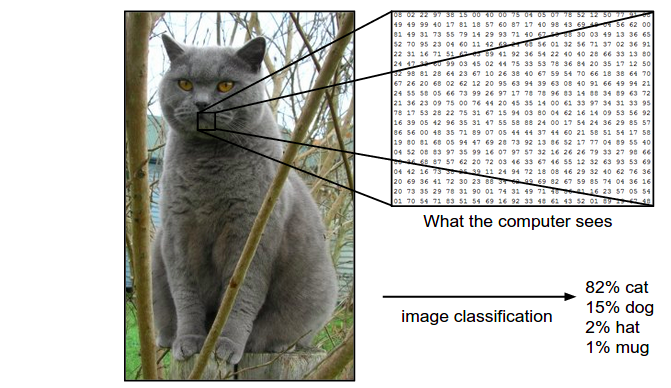
\includegraphics [scale=0.5] {cat}
	\captionof{figure}{How a computer perceives an image-source \cite{softmax}}
	\label{fig:cat}
\end{figure}

\subsection{Convolutional Layer}
The Convolutional layer will be explained using the following example, let consider the image as a magical cake of height and width say 48x48, and there is a cake cutter of size say 5x5. The cutter is used to cut the cake from the top left. The cutter is referred to as a filter in machine learning. The cutter, in this case, is also an array of numbers called weights and for the maths to work the cutter must have the same depth as our cake (5x5x3). Lets first consider the cutter being in the first position ie. the top left of the cake. The values in the cutter are multiplied by the values of the cake (element-wise multiplications). These multiplications are all summed up and result in a single number. This single number is only for the first part and this process is repeated throughout the whole cake (Next step would be moving the cutter to the right by 1 unit, then to the right again by 1, and so on) keep in mind its a magical cake so you can cut a part more than once. After using the cutter on the whole of the magical cake we result in a new cake of size 28x28x1, the results is called a feature map. The filters are low-level feature identifiers. Which identified features as it was passing through the whole cake (straight edges, simple colors, and curves). 


\subsection{Activation Functions}
The activation functions are an important part of a CovNet, they are mostly added to the output end of a Convolutional layer. They usually map the output values between 0 and 1 or -1 and 1. The activation functions can be divided into two categories; linear and non-linear functions. The non-linear functions are the most used because most of the real-world data are non-linear. There 3 main types of this function that are mostly used. They are the sigmoid, tanh and ReLu. The sigmoid map the output value between 0 and 1, the tanh maps the output between -1 and 1 and finally the ReLu the most used activation function. The Rectified Linear Units (ReLU) is found in all layers during the Convolution phase, this layer implements element-wise nonlinearity to our Convolutional layer, this just means it helps to handle situations where the relation between the input values and the CovNet output is non-linear. The ReLU has a function \(f(x) = max(0,x)\) which means if you give it a value x, it will return 0 if x is negative and will return the value itself if its positive. ReLU is mostly used because it speeds up the training process significantly and it does not saturate(the gradient is small if the input is elevated or small), unlike the tanh and sigmoid~\cite{relu}. Figure~\ref{fig:relu} shows a plot by Krizhevsky et al.~\cite{krizhevsky2012imagenet} paper, the figure shows that there is a 6x advancement in convergence with the ReLU unit compared to the tanh unit. The bold line represents the ReLU and tanh is the dashed line.

\begin{figure}
	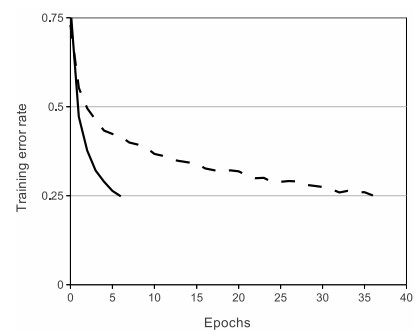
\includegraphics [scale=0.9] {relu}
	\captionof{figure}{ReLU unit compared to the tanh unit from Krizhevsky et al. paper \cite{krizhevsky2012imagenet}}
	\label{fig:relu}
\end{figure}


\subsection{Pooling Layer}
The pooling layers basically have two main functions, the first one is that they help the CovNet to locate features regardless of which part of the image the features are located. This results in the model being robust against small changes in the position of the features of the images. The second function is that it also helps to reduce the size of the feature map. Therefore computations in the futures layers are relatively less complex. One way of performing pooling is using max pooling technique other less used techniques include average and sum pooling, the idea in max-pooling is like sliding a window through the feature map, the windows fills a number of arrays in the feature map therefore, you pick the largest among all the numbers and disregard the rest of the numbers. This technique is employed in the first, second and last Convolutional layers of the AlexNet architecture.

\subsection{Dropout Layers}
The following is inspired by an article on Medium~\cite{dropout}. This layer is used for regularising your network. The dropout is used in our CovNet to prevent over-fitting. The Fully connected layers eventually handle more parameters and therefore neurons become co-dependent on one another, and this leads to over-fitting during the training phase. When dropout is implemented in a network, it does not use all neurons during a particular forward or backward pass during training but, chooses random neurons at a specified probability for each pass. Figure \ref{fig:dropout} shows a neural network with an implemented dropout and another without dropout.

\begin{figure}[!htb]
	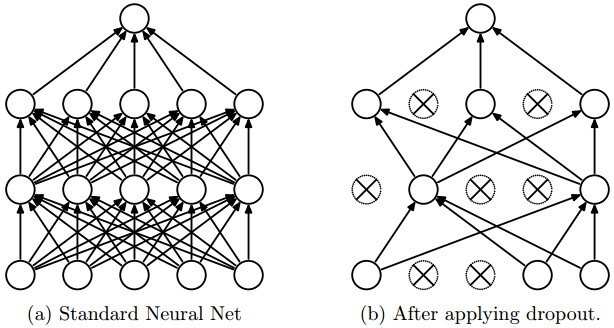
\includegraphics [scale=0.6] {dropout}
	\captionof{figure}{Left: shows a standard neural net. Right:
		shows a neural network where dropout has been applied on.
		Crossed units are dropped units. figure from Krizhevsky et al. paper \cite{srivastava2014dropout}}
	\label{fig:dropout}
\end{figure}


\subsection{Fully Connected Layer}
Fully connected simply implies that every neuron from the previous layer is connected to every other neuron in the next layer. The output of this layer are high-level features of the image presented to the network. The output of this layer is a probability distribution of all the classes in the network and this is ensured by using an activation function, usually a softmax activation function. We use a softmax activation as opposed to other activation functions because, it handles low invigoration in images (say blurry charts) of your neural net with rather uniform distribution and to high invigoration in images (say large numbers, like sharp images) with prediction probabilities between 1 and 0. To put in simple terms, the Convolutional and pooling layers act as feature extractors and the last layer, the fully connected layer act as the classifier.

\begin{equation} \label{eq:soft}
f_j(z) = \frac{e^{z_j}}{\sum_k e^{z_k}}
\end{equation}

The equation \ref{eq:soft} is a softmax function, (z) represents a vector, so the function takes (in z) and crushes it to a probability value between zero and one \cite{softmax}.

\section{Adding more steps}
The layers mentioned above are a standard for every CovNet and with this kind of setup and a good dataset, most simple experiments are most likely to turn out with good results. However, when dealing with more complex problems in real-world other strategies like stacking more Convolutional layers and adding max-pooling at some points to reduce the dimensions of your data. The more Convolutional layers your network has the more it learns complex features, but also the more computational power you need. So the question then arises, how do you know how many layers to add so as to achieve the best results with the least possible computational power? The answer to this is experimentation, a lot of experiments and testing should be done in other to get the optimal structure \cite{layers}. Another step that improves image classification is some processing of the images before passing them as input into the machine learning algorithm. In the next section, some image processing techniques performed on the dataset before feeding the images to the network are discussed.


\subsection{Image Processing Techniques}
CovNets are very powerful and have the ability to learn features with some level of spatial invariability, this ability, however, is limited when it comes to choosing parameters in an efficient manner~\cite{jaderberg2015spatial}. To further improve robustness to spatial invariance during testing, some preprocessing techniques like data augmentation are applied on the train data.

One relevant feature of CovNet is its multi-layer representation, which is responsible for the classification phase. This multi layer representation is not engineered but rather reliant on the data presented to it~\cite{van2017learning}. The multi-layer representation determines the kind of features important for the classification task. To find the right multi-layer representation, the network must be presented with a variety of instances of the image, so as to be able to capture the different appearance of the image. There are some parts of the image that can be varied and these parts are: the location, the viewpoint, and the size of an object or pattern. We, therefore, perform some preprocessing techniques in other to capture the 3 main ways images can be altered so that our model is better generalized. 

\begin{itemize}
 	\item Data Augmentation: CovNets require a large train dataset in other to learn. The formation of such a dataset is a strenuous and expensive task. Data augmenting eases this task by creating label preserving transformations samples by transforming, rotating, flipping or even scaling the original samples. This technique helps the model to be robust to changes in position and orientation ~\cite{taylor2017improving}. 
 	
 	\begin{figure}[!htb]
 		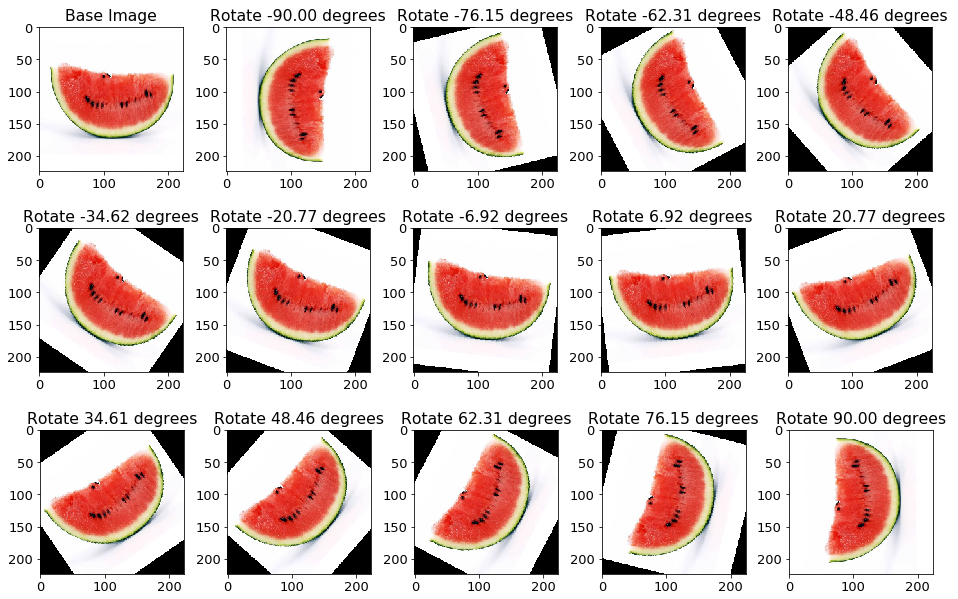
\includegraphics [scale=0.44] {augmentation.png}
 		\captionof{figure}{Data augmentaion technique of Rotation (at finer angles) source \cite{augement}}
 		\label{fig:augment}
 	\end{figure}
 
 \item Normalization: The process where the range of pixel intensity values is changed, this is done to bring the pixels to a range that our senses are more familiar to. The motivation for normalizing image data is to achieve consistency in the range of pixel values in the data. There are mainly two types of normalization techniques: the first one is Scaling, that is putting the values on the same scale and secondly centering, which involves balancing the data around a particular point. Both techniques have different benefits and should be selected based on our needs. For instance, scaling speeds up convergence and centering fights the problem of vanishing gradient~\cite{normalizing}.

\end{itemize}

\section{Validation in Machine Learning}
The following argument is based on Ricardo Gutierrez-Osuna's lecture~\cite{validation}.
Every machine learning algorithm has some parameters that can be tuned to adapt to a specific problem. For instance, in CovNets those parameters are the number of hidden layers, weights, and biases. During the training process of a machine learning algorithm, these tunable parameters are given specific configurations (model), we then check the classification performance of the algorithm with these estimated configurations. Classification performance is mostly estimated by finding the error rate of the entire dataset. We, therefore, try to tune our parameters to classify with the least error rate. In an ideal situation where our dataset consist of all possible variants of the samples to be classified, the error rate on the entire dataset will be the true error rate, but with real-world data this situation is unrealistic. The model will perform well on samples it has seen but will fail on new samples, this situation is known as over-fitting. In other to overcome this limitation some validation techniques are adapted during the training phase. These techniques are presented below.

\subsubsection{Holdout}
The holdout method involves splitting the dataset into two disjoint groups. Train set used to train the model and test set used to estimate the error rate of the model. The train to test split ratio can be a 60/40 or 70/30 or 80/20 split on the dataset. One drawback of this method is that if we have a small dataset, we cant afford to set aside a portion for testing only. Another drawback could be that if the difficult patterns end up in the test set the accuracy might be misleading.

\subsubsection{Cross-validation}
In this method the data is divided into say k subsets, the holdout method explained above is then repeated k times i.e each time one of the k subsets is used for testing and the other k-1 subsets are combined and used for training. The true error rate of the model is the average error across all the k trials performed.

\subsubsection{Leave-one-out cross validation}
The leave one out technique can be likened to the cross validation method. The main difference is that the k subsets are equal to the number of samples in the dataset. So, therefore, the model is trained on all the samples except one, and a prediction is made from that point. The true error rate, in this case, is also the average of all the k trials. The major drawback is that it can be computationally expensive.


\section{Performance Evaluation}
The following argument is based on Mohammed Sunasra's article on Medium~\cite{performance}.
After going through the process of putting together a dataset, estimating the best parameters for a machine learning algorithm, implementing a model and getting some output prediction on the classes trained on, the next step will be to find how well our model performed using some type of metrics. There exist quite a number of performance metrics that can be employed to evaluate a machine learning model. Some of these metrics that are used to evaluate classification problems are described below.

\subsubsection{Confusion Matrix}
The Confusion Matrix is an intuitive way used to describe the accuracy of a model. This metric is useful in problems where there exist multiple types of classes. A confusion matrix is a table that shows the number of correct and wrongly predicted values in each classification class. It gives insight into the type of errors being made by the classifier on each class.


\begin{table}[h]
	\centering \def\arraystretch{1.5} \small
	\begin{tabular}{|p{3cm}|p{3cm}|p{3cm}|}
		\hline
		  & class 1 \par Predicted & class 2 \par Predicted \\ \hline
		class 1 \par Actual & TP & FN \\ \hline
		class 2 \par Actual & FP & TN \\ \hline
			
	\end{tabular}
	\caption {Confusion Matrix}	
	\label{table:confusion}
	\end{table}
The numbers inside the Confusion matrix can be used to calculate 
all the performance metrics. The terms used in the table and how they are used to calculate the other metrics are explained below.

\begin{itemize}
	\item TP (True Positive): Observations predicted as positive, that are actually positive.
	\item FP (False Positive): Observations predicted as positive, but are negative.
	\item TN (True Negative): Observations predicted as negative, but are negative.
	\item FN (False Negative): Observations predicted as negative, but are positive.
\end{itemize}

\subsubsection{Accuracy}
In any classification problem, the accuracy is the number of correct predictions made overall the predictions made. Equation ~\ref{eq:accuracy} shows how the values in the confusion matrix are used to calculate the accuracy of a model. Accuracy is mainly used when there is an even number of samples in each class.

\begin{equation}
Accuracy = \frac{TP}{TP + FP + TN + FN} \label{eq:accuracy}
\end{equation}


\subsubsection{Precision}
Precision tells us if the portion of the sample in a particular class that was predicted as positive were actually positive. So it considers samples predicted as positive (TP and FP), and those that were actually positive TP. Equation~\ref{eq:precision} shows how the precision of a model is calculated.

\begin{equation}
Precision = \frac{TP}{TP + FP} \label{eq:precision}
\end{equation}

\subsubsection{Recall}
Recall or Sensitivity tries to answer the question, of all the positive samples what portion were actually identified correctly.
It considers the actual positives (TP and FN) and samples classified as positive (TP).
Equation~\ref{eq:recall} shows how the precision of a model is calculated.

\begin{equation}
Precision = \frac{TP}{TP + FN} \label{eq:recall}
\end{equation}

\subsubsection{F1 Score}
F1-score is just a way to represent both precision and recall as a single value. It is taking the harmonic mean \footnote{http://www.statisticshowto.com/harmonic-mean/} of the precision and recall of the model. Equation~\ref{eq:f1score} shows how the F1 score is calculated.

\begin{equation}
Precision = \frac{2 * Precision * Recall}{(Precision + Recall)} \label{eq:f1score}
\end{equation}

There are many other metrics used in machine learning to evaluate a model but the ones mentioned above are mostly used when it comes to classification problems.


\subsection{Deep Learning Frameworks}
This section is inspired by a blog, 10 Best Frameworks and Libraries for AI \cite{framework}.
Machine learning has become a friendlier field due to the amount of interest it has gained in recent times. Due to this interest, there has been a huge improvement and a lot of new developed libraries and frameworks. There is, therefore, a headache when choosing a framework for a particular. In this section, some of the most popular frameworks that are used for CovNets are discussed. 

\subsubsection{Theano}
Theano is a library used with python and is flexible. There also exist very good documentation free to use. It is really good with numerical operations with multi-dimensional arrays.

\begin{itemize}
	\item [\textbf{Pros}]
	\item It is optimized for CPU and GPU.
	\item Performs numerical computations efficiently.
		
	\item [\textbf{Cons}]
	\item Need to be combined with other high-level libraries like keras for better abstraction
	\item it's a low-level library 
\end{itemize}

\subsubsection{TensorFlow}
Tensorflow is built on C++ and Python programming languages and available in python. It is developed and maintained by Google developers.  It is open source and very efficient when carrying out numerical tasks using data flow graphs. Tensorflow is arguably the most used neural network framework.

\begin{itemize}
	\item [\textbf{Pros}]
	\item The inner working can be visualized with Tensorboard.
	\item Performs numerical computations efficiently.
	
	\item [\textbf{Cons}]
	\item Speed is a problem as python is not soo fast
	\item Limited access to pre-trained models
\end{itemize}

\subsubsection{Caffe}
Caffe is a very fast and efficient deep learning framework. It very easy to use especially for image classification.

\begin{itemize}
	\item [\textbf{Pros}]
	\item has great performance.
	\item you can train a model without actually writing any additional code.
	
	\item [\textbf{Cons}]
	\item does not work well with new architectures
	\item also bad for implementing with recurrent neural networks.
\end{itemize}

\subsubsection{Torch}
Torch is another open-source library that works well with scientific and numerical calculations. Torch is based on the Lua programming language. It works well with operations such as slicing and indexing since it has a potent N-dimensional array. The main disadvantage of Torch is that access to documentation is very unclear. Also, there is no readily available code we can just use.

As we have seen there is a wealth of frameworks that exist, these frameworks facilitate easier the running of deep network code. Selecting the right one for your work will depend on your requirements. Either you go for speed, handling of computational complex calculations, less computational power or memory efficient frameworks.

\subsection{Training process}
This section is inspired by a blog written by ujjwalkarn \cite{cnnonline}. In machine learning, a model is an artifact created during the training phase, this model can be likened to a function that maps specific features to their respective labels, the model is trained with a portion of the dataset called the train set. As the model is trained, the validation set is used to decide and pick which metric out of hyper-parameters, early stopping and architecture considerations yield the best performance. This helps to adjust and optimize the model~\cite{validation}. Finally, the test-set in machine learning is the other portion of the dataset which was not used during the training phase. The test-set checks how well the trained model performs on unseen data by giving an unbiased assessment of the model. Most machines learning datasets are therefore divided into train, validation and test set.
The process by which a CovNet performs classification is summarised below.

\begin{itemize}
	\item All parameters (weights, filter, and biases) are initialized randomly.
	\item The network is then given as input the image. The forward pass is then performed (convolution, ReLU, pooling and fully connected layer), the output is a probability of each class.
	\item here the error in the output is calculated.
	\[Total Error = \sum  \frac{1}{2} (target probability - output probability) ^2 \]
	\item This step reduces the total error by performing back-propagation, the gradients of the error with respect to the weights are calculated. This is used to update parameters and therefore results in reducing the total error.
	\item In the final step, steps 2 to 4 are repeated for all images in the training dataset. The best parameters are then stored for the prediction of a new image given to the network. 
	
\end{itemize} 

\section{Review of chart image Classification Techniques}
In the rest of this chapter, four related works that performed chart image classification with unique methods and also achieved good results are described in details.  

\subsection{ImageNet Classification with Deep Convolutional    Neural Networks}
The first related work is the work of Krizhevsky et al.~\cite{krizhevsky2012imagenet}. In this work, they show that a large, deep CovNet can achieve good results on complex tasks using purely supervised learning. The dataset used was the famous ImageNet Large-Scale Visual Recognition Challenge (ILSVRC) image dataset, this dataset consists of roughly 1.2 training images, 50,000 validation images, and 150,000 testing images. All images were down-sampled to a fixed size of 256 × 256. The only pre-processing technique used was centering the image and nothing else. The architecture of the CovNet comprised of five convolutional and 3 fully connected layers. Every convolutional and fully-connected layer was followed by the ReLU
non-linearity function. The first two convolutional layers are also followed by normalization layers. Max-pooling layers followed the normalization layers and the last convolutional layer. In other to reduce over-fitting, a dropout of 0.5 was used in the first and second fully connected layers. A learning rate of 0.01 which was later reduced by three times prior to termination was used. The training was set to 90 cycles and this took five to six days to train all 1.2 million images on two NVIDIA GTX 580 3GB GPUs. The results archived were better than the previous state of the art. An error rate of classifying on one of the classes considered most probable by the classifier as the top-1 was 37.5\% and top-5 error rates on 5 classes was 17.0\%.


\subsection{Machine Learning Classification Algorithms to Recognize Chart Types in Portable Document Format(PDF) Files}
Karthikeyani and Nagarajan's work ~\cite{karthikeyani2012machine} focuses on classifying charts found in pdf files. The steps employed for the classification task involves extracting texture features from the charts and then, using a machine learning technique for the classifying phase. The dataset consists of images extracted from various pdf's. The dataset is made up of 155 256*256 RGB images. Table~\ref{table:pdf} shows the details of the dataset used.
The technique used involved extracting handcrafted features from the chart image and then, using these features as input for a model to be trained and tested. For the feature extraction phase, Gray Level Co-Occurrence Matrix (GLCM) is employed. GLCM is a technique which uses co-occurrence matrix to extract texture features of an image with the use of statistical equations. GLCM was used to extract eleven features, these included: area, median, minimum and maximum intensity, contrast, homogeneity, energy, entropy, mean, variance, standard deviation, and correlation. These extracted features are correlated to the pixels of the image. These extracted features are then stored using a 2-dimensional matrix-vector data structure. This structure has thirteen (13) columns and 'x' rows, where x is the size of the dataset. The features are stored in twelve (12) columns and the label is stored in the thirteenth column. The features and labels were stored in the below structure~\ref{alg:1}.

\begin{table}[h]
	\centering \def\arraystretch{1.5} \small
	\begin{tabular}{|p{3cm}|p{3cm}|p{3cm}|p{3cm}|}
		\hline
		Chart Type & No of Charts & Chart
		Type & No of Charts  \\ \hline
		2D Bar chart & 40 & Doughnut 2D & 7 \\ \hline
		3D Bar chart & 16 & Doughnut 3D & 11\\ \hline
		2D Pie chart & 13 & Line & 35 \\ \hline
		3D Pie Chart & 20 & Mixed Chart& 13 \\ \hline
	\end{tabular}
	\caption {Details on Dataset from \cite{karthikeyani2012machine} }	
	\label{table:pdf}
\end{table}


\begin{algorithm}
\caption{This is the structure used to store the features}
\label{alg:1}
Struct FeatureVector \{\\
	float feature1; float feature2;\\
	float feature3; float feature4;\\
	float feature5; float feature6;\\
	float feature7; float feature8;\\
	float feature9; float feature10;\\
	float feature11; float feature12;\\
	int target;\\
\}
\end{algorithm}

This vector-like structure is then fed as input into three classifiers SVM, MLP neural network, and K-Nearest Neighbor. These classifiers are then trained and a classification model is formed for the recognition step. After this, to see if the model works well a test set consisting of new records is fed into the model for the model to predict their labels. Three metrics were used to check the performance of the model, these metrics are  the error rate, classification accuracy, and speed of classification. The error rates obtained were MLP 0.30, K-NN 0.22 and SVM 0.23. The scores of the accuracy metrics were KNN (78.06\%), MLP (69.68\%) and SVM (76.77\%) and finally the speed metric. The speed metric which is the sum of training and test time together was recorded with MPL having the slowest time of 8.38, followed by SVM with 0.31secs and KNN with 0.26secs. Even though these results were good, the paper proposed extracting features which are related to shape and curves since these features will carry more unique information to distinguish charts.

\subsection{Architecture proposal for data extraction of chart images using Convolutional Neural Network}
Our work is inspired by the technique used in the work of De Freitas et al.~\cite{junior2017archi}. They proposed a way to extract the raw data visualized in different chart images. The paper talks about two main stages of accomplishing this task. Firstly, the classification of charts is done since it allows the different variety of charts to be detected automatically allowing the next step, which is the extraction of data from the classified charts. The paper, however, focuses on the first step which only involves the classification of charts. In this paper, a Convolutional Neural Network is used for the classification task. The Convolutional neural network encapsulates the characterisation and classification processes during its learning process, unlike other old techniques. The dataset used for this task were searched and downloaded by using Google image search. Table~\ref{table:rela} shows the chart types which were collected and the number of train and test sets which the respective charts were divided into.

\begin{table}[h]
	\centering \def\arraystretch{1.5} \small
	\begin{tabular}{|p{5cm}|p{3cm}|p{3cm}|}
		\hline
		Chart Type & Test & Train \\ \hline
		Area Chart & 50 & 555 \\ \hline
		Bar Chart & 50 & 657 \\ \hline
		Line Chart & 50 & 489 \\ \hline
		Map & 50 & 476 \\ \hline
		Pareto Chart & 50 & 261 \\ \hline	
		Pie Chart & 50 & 361 \\ \hline
		Radar Chart & 50 & 454 \\ \hline
		Scatter Chart & 50 & 552 \\ \hline
		Table & 44 & 236 \\ \hline
		Venn Diagram & 48 & 304 \\ \hline
		Total & 498 & 4345 \\ \hline
		
	\end{tabular}
	\caption {Number of Train and Test Dataset collected}	
	\label{table:rela}
\end{table}

For the classification, a variant of CovNet called LeNet-based CovNet model is used. The model was implemented using Tensorflow\footnote{https://www.tensorflow.org/}, LeNet-based CovNet has an architecture which is comprised of 3 convolutional layers, followed by a fully connected layer. The model is trained in a way that the dataset is divided into mini-batches, samples of fixed sizes(100) are selected and fed into the CovNet, as a result of this process the model becomes robust since it learns to generalize from the different min-batches which are fed into the model. Also, all the images are converted to jpeg and resized to 224x224x3, that is, 224 pixels of height, 224 of width and 3 layers of output. The other parameters used were 1000 epochs and a learning rate of 0.003. The accuracy at the end of the training process was 70\% which is pretty decent.

\subsection{Chart classification by combining deep convolutional networks and deep belief networks}
In another paper by Liu et al.~\cite{liu2015chart}, a new approach was proposed for the process of chart classification. The process involves using CovNet to extract deep hidden features of charts and then employing a deep belief network to use the extracted features to predict the labels of the charts. Due to a difficulty in acquiring a large number of charts as training data, the famous ImageNet model trained with 1.2 million natural images was retrained with just over 5,000 collected charts images. The types of charts collected were pie charts, scatter charts, line charts, bar charts, and flowcharts. The architecture of the CovNet used is made up of five Convolutional layers, two fully-connected layers, and an output layer. The preprocessing steps for the images involve down-sampling them to 256 x 256 x 3, after which each is cropped to a size 227 x 227 from the center and its horizontal flip is extracted as the input of the CovNet, other parameters used for the CovNet include a learning rate that starts with 0.01 initially and later decreased by a factor of 0.1 after every lOOk iterations, the weight decay parameter was set at 0.0005 and a dropout rate of 0.5. This results in an output of a 5-way softmax which produces the distribution over the 5 class labels and this is used as input for the deep belief network. The deep belief network architecture has three hidden layers, whose dimensions are 5000, 500 and 2000. This results in a softmax predicting the probability distribution over the 5 categories of charts as output. The training process was done with 4000 randomly selected images and the rest were used as test set. The accuracy of the model after the evaluation was 75.4\%. Table~\ref{table:deep} shows the results gained. It shows the results after the training was done pre-trained with the natural images without deep belief networks, and also shows the results gained when the training was done with only the chart dataset but with deep belief networks.

\begin{table}[h]
	\centering \def\arraystretch{1.5} \small
	\begin{tabular}{|p{3cm}|p{3cm}|p{3cm}|p{3cm}|}
		
		\hline
		Chart & CovNets&CovNets+DBN without pre-training & CovNets+DBN \\ \hline
				
		Bar Chart & 75.6\% & 45.6\% & 74.2\% \\ \hline
		Flow Chart & 88.3\%  & 56.8\% & 91.3\%  \\ \hline
		Line Chart  & 71.2\%  & 22.3\% & 67.9\% \\ \hline
	
		Scatter Chart & 69.8\% & 44.5\% & 84.2\% \\ \hline
		Pie Chart & 58.1\%  & 50.1\% & 59.4\%    \\ \hline
		Ave. Accuracy & 72.6\%  & 43.9\% & 75.4\% \\ \hline
		
	\end{tabular}
	\caption {Comparing Results of Proposed Framework from (Liu et al.~\cite{liu2015chart}) }	
	\label{table:deep}
\end{table}


\section{Summary}
This chapter discussed the background literature on chart image classification. The two main approaches to chart images classification were mentioned first. In Section 2.3 and 2.4, the model-based and machine learning approaches were explained. In Section 2.5, CovNet a machine learning approach used commonly for visual image recognition is reviewed and discussed, also some additional step like image processing techniques that improve image classification are mentioned and discussed in Section 2.6.  In Section 2.7 validation techniques to help choose the tunable parameters in a machine learning algorithm are discussed. In Section 2.8 some performance evaluation metrics that help us know how well a model is performing are presented and discussed. Towards the end of this chapter, some related works that inspired this thesis were discussed.


\chapter{Approach}

\section{Overview}
In this chapter we present the proposed approaches used in this thesis for chart image classification. As discussed in the previous chapters, the proposed approaches involve two main steps, namely, the image processing step and classification step. How the dataset was created is discussed in section 3.2 and Section 3.3. In Section 3.4 the process which the train, validation and test data are acquired are discussed. In Section 3.5 the proposed architecture and important parameters of the CovNet is discussed. The processing techniques used for the images are discussed in Section 3.6. Lastly,the various parameters used for the training of the network is discussed.\\\\

\section{Dataset}
The following paragraph is inspired by a blog written on what to look for in training data~\cite{edi}.
The saying 'Garbage in Garbage out' is a valid statement when it comes to creating a dataset for machine learning. The machine learning technique will learn from whatever data fed to it. So if a dataset of good quality is fed into the algorithm, then the model created will also be of good quality. The dataset creation stage is therefore an important stage. In most approaches that worked on chart images classification, the dataset used consisted of chart images downloaded from Google and a few others were obtained from extracting chart images from pdf's. This approach we believe is limited since, we don't know the programming languages, the libraries used and parameters used in creating these charts. This missing information is relevant since it tells us how diverse our resultant dataset is. For example, how are we sure that all the charts that were downloaded from Google, were not only created in Python or Java?, and in such a case how well will a new chart created with Matlab or R be classified. For this reason the dataset comprised of image charts created with different libraries and with dissimilar programming languages. Some random chart images from other works were manually labeled and added to our created dataset. In the next sections, the various datasets and the languages used in plotting are described. To make the dataset as diverse as possible, charts created in each programing language used a different set of CSV files. 

\subsection{Dataset for Matlab}
The Data used for creating the plots in Matlab were randomly chosen from Project Dataset \cite{projectdataset}, a free CSV data repository, DatPlot \cite{datplot} and Plotly CSV repository in github \cite{plotly}. The datasets are multidimensional and compiled from normal day to day activities like dating, what makes people happy etc, and objects like cameras and cars. On the average the datasets used contain about 500 instance and 5 different columns. The biggest dataset is called Speed dating data. It is made up of over 8,000 observations of answers to survey questions about how people rate themselves and how they rate others on several dimensions. The smallest dataset used has 33 instances and 12 columns. It contains information about cars. The number of gears and speed, just to name a few attributes.

\subsection{Dataset for R}
For the plots in R, 13 random CSV files where downloaded from an archive of datasets distributed with R called Rdatasets  \cite{rdata}. Rdatasets is a collection of dataset distributed with R. On the average there are 80 instances and 5 columns in each dataset.
The biggest CSV file is the Australian athletes dataset. It's made of 203 instances and 14 columns and contains attributes like sex,height,weight and sports. The smallest dataset is the Canadian Women's Labour-Force Participation. This dataset has 30 rows and 7 columns. It contains information like average wages of women, percent of adult women in the workforce etc.


\subsection{Dataset for Python}
The data used for creating the plots in Python were 15 randomly seleted csv files also from  Rdatasets \cite{rdata}. The biggest dataset among the 15 is the Monoclonal gammapothy data, it contains natural history patients with monoclonal gammapothy of undetermined significance. The dataset is made up of 1384 observations with 10 columns, it has attributes like age, sex, time of death and last contact in months. On the average each dataset contains about 200 instances and 7 columns of multi-dimensional data. The smallest dataset however contains only 33 instances with 11 columns and is called the Nuclear Power Station Construction Data.The data relate to the construction of 32 light water reactor (LWR) plants constructed in the U.S.A in the late 1960's and early 1970's.

\subsection{Dataset for Java}
For the plots created in java, I used the dataset made available by Plotly \cite{plotly}, a github repository of CSV datasets used in the Plotly API examples. 14 random CSV files were downloaded, the biggest file has 1002 instances and 9 columns, and on the average each file contains about 100 instances and 9 columns. The smallest file however is made of 33 instances and 12 columns called the mtcars file. It contain information about a variety of different car models like the number of gears, speed etc. The table \ref{table:1} contains the names of all CSV files that were used in the different languages with the different plotting programs.


\begin{table}[!htbp]

	\centering
	
\begin{adjustbox}{max width=1.1\textwidth,center}
	
	\begin{tabular}{|p{5cm}|p{3cm}|p{3cm}|p{4cm}|}
		
		 \hline
		 \multicolumn{4}{|c|}{Datasets} \\
		 \hline
				
		Python & Matlab & R  & Java\\ \hline
		
		3d\_line\_sample\_data.csv \par LightFordwardFlapStall.csv  \par line\_3d\_dataset.csv \par
		longley.csv  \par loti.csv  \par lung.csv  \par nuclear.csv  \par timeseries.csv  \par
		USJudgeRatings	\par WVSCulturalMap.csv  \par wind\_rose.csv  \par volcano.csv  \par uspop2.csvm \par tips &
		
		Camera.csv \par Cars.csv \par speedDating.csv \par Cereal.csv  \par happiness.csv \par TestData1.csv \par TestData2.csv  \par mpg.csv \par okcupid-religion.csv  \par spectral.csv
		\par stockdata.csv \par subplots.csv  & 
		
		ais.csv \par Angell.csv  \par Baumann.csv \par Bfox.csv \par cane.csv \par carprice.csv \par Chirot.csv
		Davis.csv \par Ericksen.csv \par Florida.csv \par Highway1.csv \par Pottery.csv \par Prestige.csv 
		salinity.csv \par urine.csv & 
		
		3d-line-plot.csv \par 3d-scatter.csv \par 2011\_flight\_paths.csv \par 2011\_us\_exports.csv \par auto-mpg.csv \par candlestick\_dataset.csv \par finance-charts-apple.csv \par 
		globe\_contours.csv\par hobbs-pearson-trials.csv \par motor\_trend\_tests.csv \par 
		nz\_weather.csv \par volcano.csv \par iris.csv \par mtcars.csv	\\ \hline
		
	\end{tabular}
	
\end{adjustbox}


\caption {Names of datasets used in each plotting program}	
\label{table:1}
\end{table}


\section{Creating Plots}
The motivation for creating a variety of plots to capture all type of plots used in scientific papers was acquired by inspecting the datasets of Architecture proposal for data extraction of chart images using CovNet paper \cite{junior2017archi} and Viziometrics: Analysing visual information in the scientific literature \cite{lee2018viziometrics}. Scripts in various languages were written to handle the plotting and labeling process automatically. All datasets for a particular plot (example scatter plot for python) are put into one folder. The scripts reads each CSV file column by column while creating the plots.
Table \ref{table:paratable} describes how the plots where created in each language. The type column describes the different variety of a particular plot, for example bar charts can be of type stacked, grouped, vertical and horizontal bar charts, also scatter plots types can be a scatter plot consisting of one type of marker, one scatter plot with multiple markers and finally a scatter plot with a line showing the correlation between the plots. 
Figure \ref{fig:bars} shows two different types of bar charts. Figure \ref{fig:bar1} is a stacked bar chart and  Figure \ref{fig:bar2} a normal vertical bar chart.
The Library column shows the different plotting libraries used, the parameter column describes parameters that were changed and finally the number of plots created were also added. The images below the tables are sample images that exist in our dataset of created plots for each language.

	
\begin{table}[!htbp]
	\centering \def\arraystretch{1.5} \small
	\caption {Overview of the varied parameters and libraries used for creating plots in the different plotting programs}	
	\label{table:paratable}
	\begin{adjustbox}{max width=1.1\textwidth,center}
				
	\begin{tabular}{|p{2cm}|p{2cm}|p{3cm}|p{4cm}|} \hline
				
\multirow{10}{*} {\rotatebox{90}{\textbf{Scatter plot}}}  &
		
			Language & Library & Parameters \\ \cline{2-4}
		
	& Python & Matplotlib v2.1.2 \par Plotly v2.5.1 \par Seaborn v0.8.1 & MarkerStyle \par 
	['o', '*', '.', '+','x']  \\  \cline{2-4}	 
		  
	& MATLAB & Default \par Plotly &  MarkerStyle \par ['o', '*','+','x','s']  \\ \cline{2-4} 
		
	& R  & Plotly \par Lattice \par Ggplot2 &  MarkerStyle \par ['o', '*', '+','x','s'] \par geom\_point(shape(1,2,16), size  (3-4)) \\ \cline{2-4}
	
	& JAVA & XChart 3.5.1\par jfreechart 1.0.1 & MarkerSize (15 -18)  \\ \hline
		
	\multirow{10}{*} {\rotatebox{90}{\textbf{Bar charts}}}  & Python & Matplotlib v2.1.2 \par Plotly v2.5.1 \par Seaborn v0.8.1 &   \\  \cline{2-4} 
		
		& MATLAB & Default &  Width of bar(14-16) \\ \cline{2-4} 
		
		& R & Default,Plotly \par R Library \par ggplot2 & space (0-3)  \\ \cline{2-4} 
		
		& JAVA  & XChart 3.5.1 \par jfreechart:1.0.192 \par javafx.scene & PlotOrientation \par (vertical or horizontal) \par with error bars \\ \hline 
			
	\multirow{10}{*} {\rotatebox{90}{\textbf{Line chart}}}	 & Python & Matplotlib v2.1.2 \par Plotly v2.5.1 \par Seaborn v0.8.1 & Linestyle \par ['-', '--', '-.', ':']   \\ \cline{2-4} 
			
		& MATLAB  & Default\par Plotly &  MarkerStyle \par ['o', '*', '.', '+','x','s'] \par markersize [8-10] \\ \cline{2-4} 
			
		& R & Default,Plotly \par R Library \par ggplot2 & \\ \cline{2-4} 
			
		& JAVA & XChart 3.5.1 \par javafx \par JFreeChart & MarkerSize (12-16) \\ \hline
			
	\multirow{9}{*} {\rotatebox [origin=c]{90}{\textbf{Box Plots}}} & Python  & Matplotlib v2.1.2 \par Plotly v2.5.1 \par Seaborn v0.8.1 &  \\ \cline{2-4}  
				
		&  MATLAB   & Default &  \\ \cline{2-4} 
				
		& R & Default,Plotly \par R Library \par ggplot2  &  \\ \cline{2-4} 
		& 	JAVA   & XChart 3.5.1 \par Jfree \par smile & LegendPosition (topleft,topright)  \\ \hline
	\end{tabular}
\end{adjustbox}

\end{table}

\begin{table}[!htbp]
	\centering \def\arraystretch{1.6} \small

	\begin{adjustbox}{max width=1.1\textwidth,center}
		\begin{tabular}{|p{3cm}|p{3cm}|p{4cm}|}
			\hline
			\multicolumn{3}{|c|}{Scatter Plots} \\
			\hline
			
			Language & Number of plots  & Type\\ \hline
			Python & 1165 &  \multirow{4}{*} {\shortstack { Unique markers, \\ With legends,\\ multiple markers \\ regplot }} \\ \cline{1-2}
			
			Matlab &  1008  &   \\  \cline{1-2}
			
			R  & 1009  &  \\	\cline{1-2}
			
			Java &  1002 &  \\ \hline
			
			\multicolumn{3}{|c|}{Bar Charts} \\	\hline
			
			Language &  Number of plots & Types(bar)  \\ \hline
			
			Python &   1018 &  \multirow{4}{*} {\shortstack {Horizontal and Vertical, \\ Stacked, \\ Grouped bar charts \\ Error bars }} \\ \cline{1-2}	 
			
			Matlab &  1063  &  \\ \cline{1-2}
			
			R &  1022  & \\ \cline{1-2}
			
			Java  &  1143 & \\ \hline
			
			\multicolumn{3}{|c|}{Line Charts} \\
			\hline
			
			Language & Number of plots & Types(Line with)  \\ \hline
			
			Python & 1019 &  \multirow{4}{*} {\shortstack { Markers, \\ Multiple Lines }} \\ \cline{1-2}	 
			
			Matlab   & 1013 &  \\ \cline{1-2}
			
			R &  1132  & \\ \cline{1-2}
			
			Java & 1089 & \\ \hline
			
			\multicolumn{3}{|c|}{Box Plots} \\
			\hline			
			Language & Number of plots & Types(Box with)  \\ \hline
			
			Python  &  1012 &  \multirow{4}{*} {\shortstack { Notches, \\ Multiple Boxes }} \\ \cline{1-2}	 
			
			Matlab   &  1032  &  \\ \cline{1-2}
			
			R & 1113  & \\ \cline{1-2}
			
			Java   & 1036 & \\ \hline
			
		\end{tabular}
		
	\end{adjustbox}
		\caption {Overview of the number of plot and different varieties plots in the different plotting programs}	
	\label{table:less}
\end{table}

\begin{figure}[!htb]
	\begin{subfigure}{.6\textwidth}
		\centering
		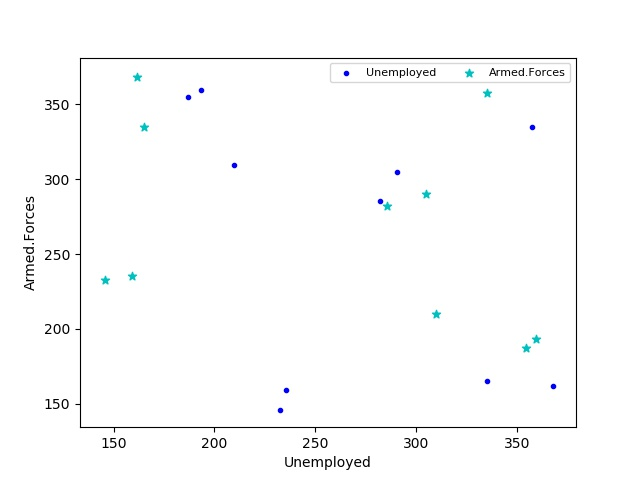
\includegraphics[width=.9\linewidth]{scatter1}
		\caption{Matplotlib scatter plot with star and circular markers }
		\label{fig:scatter1}
	\end{subfigure}%
	\begin{subfigure}{.5\textwidth}
		\centering
		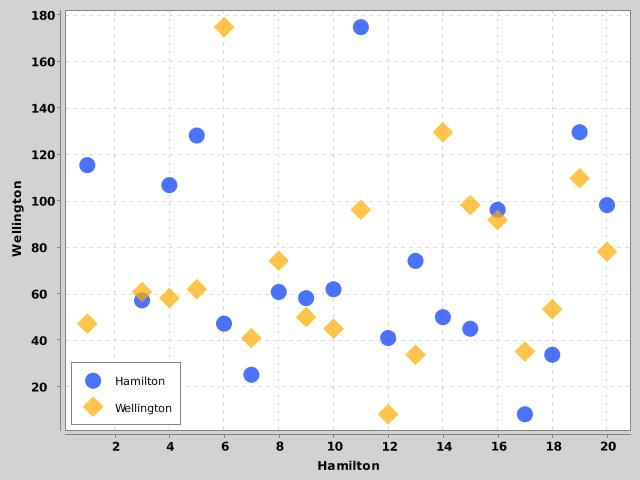
\includegraphics[width=.9\linewidth]{scatter2}
		\caption{Java scatter plot with circular and diamond markers}
		\label{fig:scatter2}
	\end{subfigure}
	\caption{Scatter plots}
	\label{fig:scatters}
\end{figure}


\begin{figure}[!htbp]
	\begin{subfigure}{.5\textwidth}
		\centering
		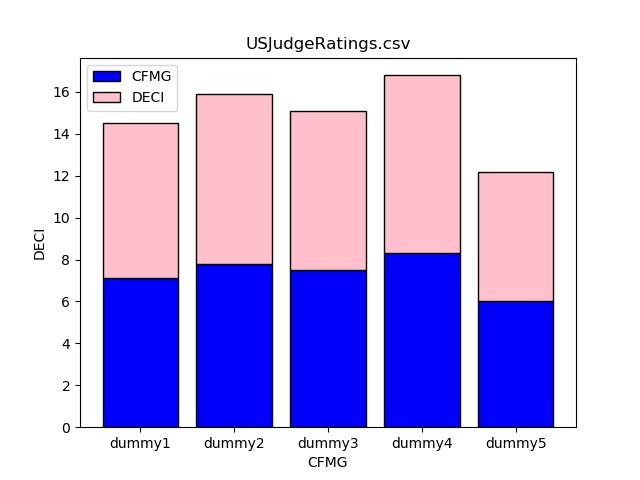
\includegraphics[width=.8\linewidth]{bar1}
		\caption{Matlab stacked bar chart (bar width 16) }
		\label{fig:bar1}
	\end{subfigure}%
	\begin{subfigure}{.5\textwidth}
		\centering
		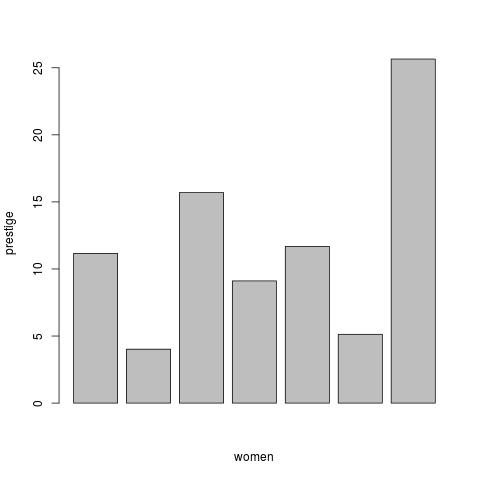
\includegraphics[width=.8\linewidth]{bar2}
		\caption{R horizontal bar chart (bar width 16)}
		\label{fig:bar2}
	\end{subfigure}
	\caption{Example Bar Charts}
	\label{fig:bars}
\end{figure}


\begin{figure}[!htbp]
	\begin{subfigure}{.5\textwidth}
		\centering
		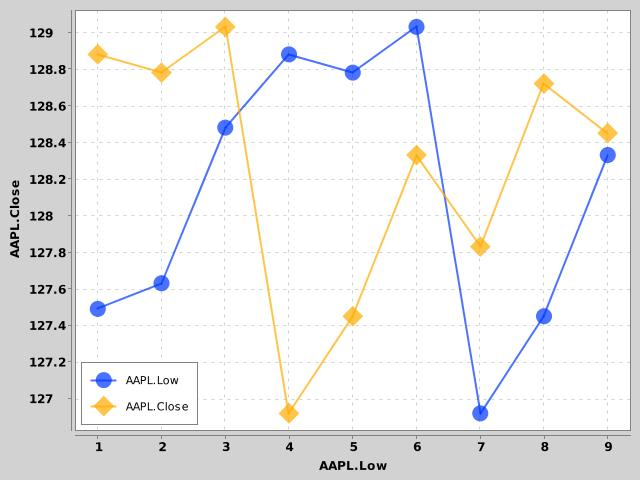
\includegraphics[width=.8\linewidth]{line1}
		\caption{Java line chart with diamond and circular markers }
		\label{fig:line1}
	\end{subfigure}%
	\begin{subfigure}{.5\textwidth}
		\centering
		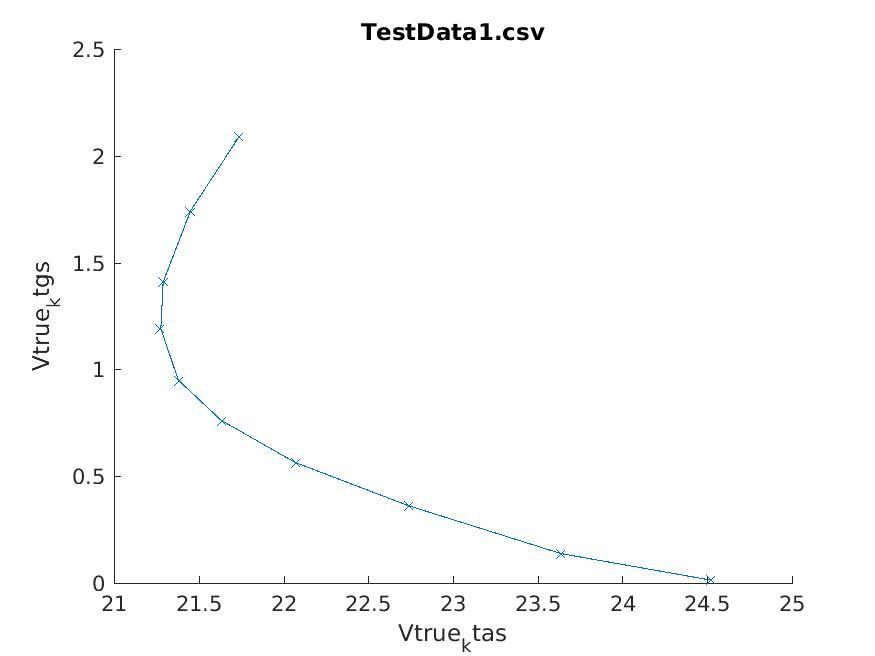
\includegraphics[width=.8\linewidth]{line2}
		\caption{simple Matlab line chart with Asterix marker}
		\label{fig:line2}
	\end{subfigure}
	\caption{Example Line Charts}
	\label{fig:figline}
\end{figure}


\begin{figure}[!htbp]
	\begin{subfigure}{.5\textwidth}
		\centering
		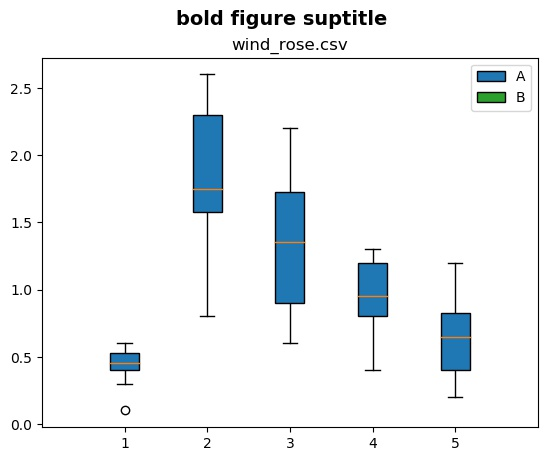
\includegraphics[width=.8\linewidth]{box1}
		\caption{Vertical multiple boxplots in python}
		\label{fig:box1}
	\end{subfigure}%
	\begin{subfigure}{.5\textwidth}
		\centering
		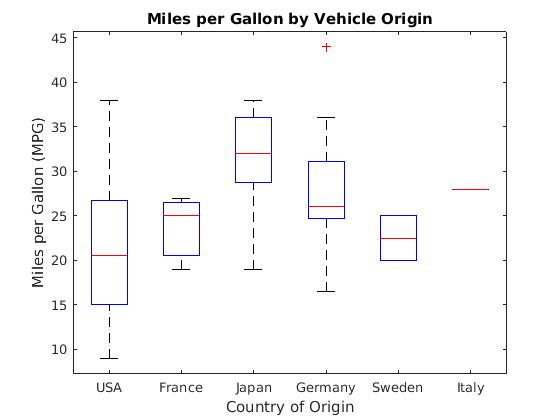
\includegraphics[width=.8\linewidth]{box2}
		\caption{Vertical multiple boxplots in Matlab}
		\label{fig:box2}
	\end{subfigure}
	\caption{Example Box Plots}
	\label{fig:figbox}
\end{figure}


\subsection{Random Charts}
In other to have the most diverse dataset, so as to achieve a robust model, we decided to pick 120 random images for each chart type  from Junior et al. \cite{junior2017archi} and Po-shen et al. \cite{lee2016viziometrix}. The line-charts, bar-charts and, scatter-plots were already labeled and were taken from the research of Junior et al. and the box-plots which we had to label manually, were taken from the work of Po-shen et al. since, the prior did not contain box-plots. The randomly picked chart images, were then added to the already created dataset for training and testing. Figure \ref{fig:random} shows sample images from the already created chart images from the paper of Po-shen et al. and Junior et al.

\begin{figure}[!htbp]
	\begin{subfigure}[b]{0.5\textwidth}
		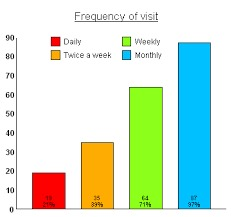
\includegraphics[width=\textwidth]{rand1}
		\caption{A bar-chart}
		\label{fig:rand1}
	\end{subfigure}
	%
	\begin{subfigure}[b]{0.5\textwidth}
		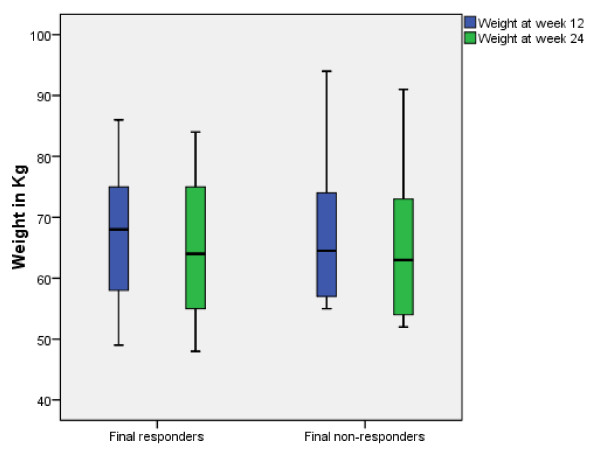
\includegraphics[width=\textwidth]{rand2}
		\caption{A box-plot}
		\label{fig:rand2}
	\end{subfigure}

	\begin{subfigure}[b]{0.5\textwidth}
		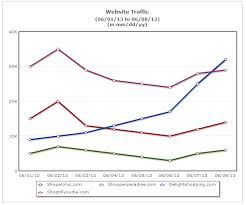
\includegraphics[width=\textwidth]{rand3}
		\caption{A line-chart}
		\label{fig:rand3}
	\end{subfigure}
	%
	\begin{subfigure}[b]{0.5\textwidth}
		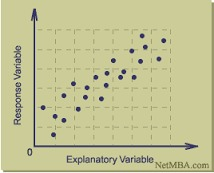
\includegraphics[width=\textwidth]{rand4}
		\caption{Scatter-plot}
		\label{fig:rand4}
	\end{subfigure}
	\caption{Example Chart images from Po-shen et al. and Junior et al.}
    \label{fig:random}
\end{figure}



\section{Training, Validation and Test set}
Figure ~\ref{fig:approach} summaries how our dataset was created and split into various portions for the training and testing stages. After creating the various plots. 80\% of each class was randomly chosen as train data and the rest was used as test data.
Also 96 of the 120 random chosen charts mentioned in the previous section was randomly picked and added to their respective classes in the train set, and the rest of the 24 which forms 20\% were added to their respective test samples.
For the validation phase, 20\% of the train set is split randomly for validation during the training phase. 
Table \ref{table:chart summary} shows a summary of how many samples were added to each class for training and testing.

\begin{figure}[!htbp]
	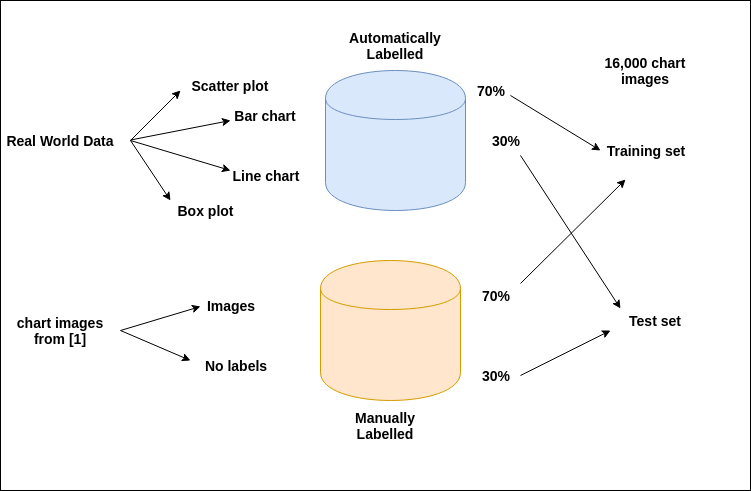
\includegraphics [scale=0.5] {approach}
	\captionof{figure}{How the train and test dataset was created}
	\label{fig:approach}
\end{figure}


\begin{table}[!htbp]
	\centering \def\arraystretch{1.6} \small
	
	\begin{adjustbox}{max width=1.1\textwidth,center}
		\begin{tabular}{|p{5cm}|p{5cm}|p{5cm}|}
			\hline						
			&Train set&Test Set  \\ \hline	 
			Scatter plot & 3442 & 862  \\ \hline
			Bar Chart & 3491 & 875 \\ \hline
			Line Chart & 3497 & 876 \\ \hline
			Box plot & 3448 &  866\\ \hline	
			Total & 13878 &  3479 \\ \hline		
		\end{tabular}
		
	\end{adjustbox}
	\caption {Summary of the dataset used for training the classifier}	
	\label{table:chart summary}
\end{table}



\section{The Architecture}
As mentioned in previous sections, our model is trained with a CovNet. The architecture of the CovNet used is inspired by the famous AlexNet CovNet architecture~\cite{krizhevsky2012imagenet}. The AlexNet architecture was used in the famous ImageNet LSVRC-2010 contest to classify 1.2 million into 1000 classes, the results obtained on the test-set had a top-5 error rate of 17.0\%, which was better than the previous state of the art. Our CovNet architecture just like the AlexNet architecture contains 8 learned layers, these 8 layers are made up of five Convolutional layers and 3 fully connected layers. A Relu is used after some Convolutional layers and fully connected layers. Another parameter employed in our architecture is a dropout, a dropout is applied in the first and second fully connected layers of our network and finally, max pooling is applied in some of the layers. A summary of our CovNet architecture used to train our model is shown in Figure~\ref{fig:archi}. The preprocessing steps, the parameters used, and why they were employed are explained into details in the rest of this chapter.

\begin{figure}[!htbp]
\centering
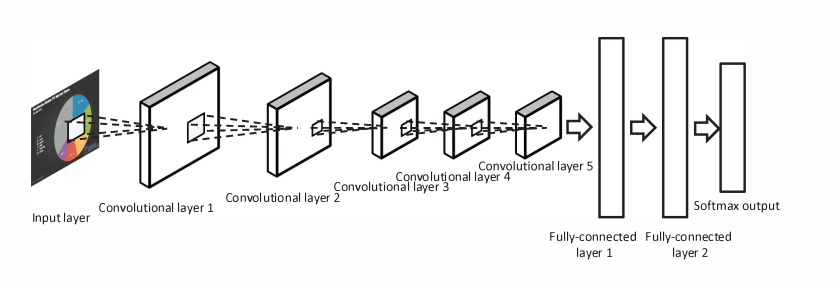
\includegraphics [scale=0.5] {architectur}
\captionof{figure}{Architecure of CovNet used to train our model source \cite{liu2015chart}}\label{fig:archi}
\end{figure}

\section{Preprocessing Techniques}
Archiving high performance by any machine learning technique is reliant on the quality and quantity of the data fed into the network.
Datasets must comprise of diverse data, this helps the network to generalise well during the testing phase. To help increase the quantity and also generate more diverse data we employ data augmenting techniques. The preprocessing techniques used in this thesis are described in the rest of this section.

\begin{itemize}
	\item  Image Resizing: The images have varying sizes and due to the presence of fully connected layer, we resize all the images to the size of 227 x 227. With this fixed image size processing in the dataset in batches is also possible.
	
	\item  Padding: Padding=Same was used while training, so that the output dimensions is equal to the input.
	
	\item  Image Scaling: All images were rescaled by a factor of 1.0/255, to enable the network to handle the images in the same way.
	
\end{itemize}

\subsection{Data Augmentation}
In this thesis, no data augmentation techniques were used. This mainly because we do not expect our images to be presented in different angles and under different lighting conditions as real world images are normally presented. This is due to the fact that images are expected to be extracted with a pdf extractor and all the bounding boxes of the chart images are expected to be horizontally aligned.  

\section{First Method}
As mentioned above the network has 8 layers, 5 of this layers are used in our architecture, and these are responsible for extracting the  features of the chart images. Our input image size used is 277 x 277 x 3  since its an RGB image, this is fed into our first Convolutional layer, this filters the image with a stride of 4 pixels. The second Convolutional layer takes as its input the output of the first Convolutional layer, between this two layers max-pooling is performed to reduce the size of the image. The third and fourth Convolutional layers, unlike the previous two have no max-pooling applied between them. The final Convolutional layer then takes as input the output of the previous layer and performs a max-pooling. The features after they are pooled are flattened to 1D vector by the flatten layer before sent to the fully connected layers. The output of this layer is then fed as input into the second fully connected layer. The output of the second layer is then fed into the last fully connected layer. The last layer in this set of 3 layers uses the softmax activation to give our output prediction. The output is a separate probability of our four classes and the choice with the highest probability is our chosen prediction. A dropout was used in the first and second Fully connected layers in our architecture. We set dropout probability to 0.5 in our network, this means nodes are dropped out with a probability of 1-05 or maintained at a probability of 0.5. Other parameters used is a learning rate 0f 1e-4 and epoch size of 3500. Table \ref{table:para} summaries the important layers and the values assigned to them.

\begin{table}[!htbp]
	\centering \def\arraystretch{1.5} \small
	\label{table:para}
	\begin{adjustbox}{max width=1.1\textwidth,center}
		
		\begin{tabular}{|p{3cm}|p{3cm}|p{3cm}|p{3cm}|}
			\hline	
			Operation & Filter & Depth & Stride \\ \hline
			
			Conv1 + Relu  &  11 * 11  & 96  & 4 \\  \hline	 
			
			Max Pooling & 3 * 3  &  & 2 \\ \hline	   
			
			Conv2 + Relu & 5 * 5 & 256  & 4 \\ \hline	
			
			Max Pooling & 3 * 3 & & 2 \\ \hline
			
			Conv3 + Relu & 3 * 3 & 384 & 4 \\ \hline	
			
			Conv4 + Relu & 3 * 3  & 384  & 4 \\ \hline	
			
			Conv5 + Relu & 3 * 3  & 256 & 4 \\ \hline	
			
			Max Pooling & 3 * 3 & & 2 \\ \hline
			
			Dropout(rate 0.5) &  & & \\ \hline
			
			Fc6 + dropout 0.5 + ReLU & & 4,096 & \\ \hline
			
			Fc7 + dropout 0.5 + ReLU & &  4,096 & \\ \hline
			
			\multicolumn{4}{|c|}{
				Fc8  + softmax output} \\
			
			\hline
			
		\end{tabular}
		
	\end{adjustbox}
	\caption {The parameters used in the AlexNet with some modifications. The order of layers is the order in which
		data is passed through. depth is the amount of output feature maps or neurons, filter is kernel
		size}	
\end{table}

\section{Second Method}
For the second experiment, the transfer learning technique used in the work of Liu et. al~\cite{liu2015chart} was employed. We used a model pre-trained by google called the MobileNet \footnote{https://ai.googleblog.com/2017/06/mobilenets-open-source-models-for.html}. MobileNet was chosen because of its small size and less computational power needed to run. The MobileNet\_0.50\_224 model was the version used for this thesis. The MobileNet model was trained with 1.2 million images with 1000 classes from the ILSVRC-2012-CLS image classification dataset~\cite{ILSVRC15}. Some of the classes in this dataset are rule, zebra, Dishwasher and dalmatian.\newline

For the training process a retrain python script originally developed by the TensorFlow authors for the purpose of using your images to train was used. The retrain scripts downloads the MobileNet model, adds a new model and retrains the new model with the chart image dataset we created. The scripts is customizable and below are the parameters we customized.

\begin{itemize}
	
	\item The validation\_percentage parameter is the part of the dataset used for validation and 20\% was used for this thesis.
	
	\item testing\_percentage parameter is the part of the dataset used for testing of final model and 20\% was used for this thesis.
	
	\item test\_batch\_size=-1 was chosen, which means all the images in reserved for testing was used.
	
	\item print\_misclassified\_test\_images:  was used so that the misclassified images where shown.
	
	\item how\_many\_training\_steps is number of epochs the nework should run and 200 was used in this thesis.
	
	\item learning\_rate: This is something you’ll want to play with. I found 0.0001 to work well.
	
	\item validation\_batch\_size: It was Set to -1, this tells the script to use all our data reserved for validation to validate on.
\end{itemize}

\section{Summary}
In this chapter we discussed our approach to classifying chart images. How our dataset was created and which raw data samples were used to create our chart images was discussed initially. In section 3.4 we discussed how the full dataset was split into train, validation and test sets for the experiments to be performed. We then talked about our modification of the AlexNet architecture used for our model training. Afterwards, the preprocessing techniques used on the dataset was explained and finally the two methods employed for classifying our model was explained in section 3.7 and 3.8.


\chapter{Experimental Results}

 \section{Overview}
This chapter presents the results of the experiments performed in the previous chapter. We answer the research question
``How Well Can We Classify the Four Different Types of Plots (Line-Charts, Bar-Charts, Scatter-plots, and Box-plots) in Scientific Literature? '' by presenting the results obtained after the experiments were performed. In Section 4.2 we present various metrics on the first methods used and Section 4.3 shows the results obtained in the second experiment.

\section{Results of First Experiment}
For the first experiment we choose different epochs sizes in other to archive good results without over-fitting. We first started with 1000 epochs, the results obtained for 1000 epochs was an accuracy of 46.8\%, out of 3478 test samples 1627 were classified correctly. We then trained our model with an epoch size of 3000, the accuracy increased to 85.9\% with 489 misclassified instances. Since our model was still not over-fitting the epoch size was increased to 3500. The accuracy of our model for training and validation was 93.8\% and 96.9\% respectively. An accuracy of 89.5\% was archived with only 365 misclassified samples was recorded on the test set. These values mean our model performs and also generalizes well.
Figure \ref{fig:matrics} shows the precision, recall and F1 measure of the results obtained after the experiments. What is interesting about this figure is that scatter plots predicted in many cases but a lot of the predictions where actually not scatter plots. So scatter plots had the most misclassified samples. Also even though line plots were predicted correctly in less instances most of the predictions were right. Bar chart and Box plots both had good number of correctly predicted instances.

\begin{figure}[!htbp]
	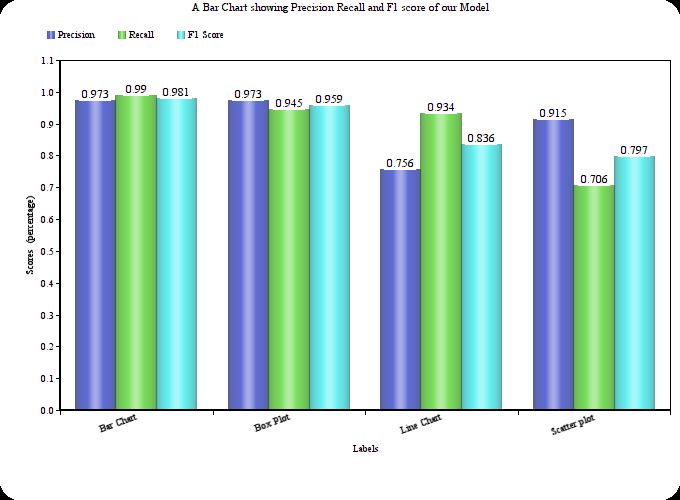
\includegraphics [scale=0.78] {scores.png}
	\captionof{figure}{A bar chart showing the precision recall and F1 scoreof our experiment}
	\label{fig:matrics}
\end{figure}

Figure \ref{fig:confusion} shows a heat map derived with a confusion metrics. 0 stands for the bar chart, 1 stands for box plot, 2 for line plot and 3 for scatter plot. Again we can see that bar charts where mostly classified correctly followed by box plot and line charts in that order and finally scatter plot were the least classified correctly. Some interesting observations were that most of the line charts were misclassified as scatter plots, a lot of scatter plots were misclassified as line charts  
and lastly, most box plots were misclassified as line charts.

\begin{figure}[!htbp]
	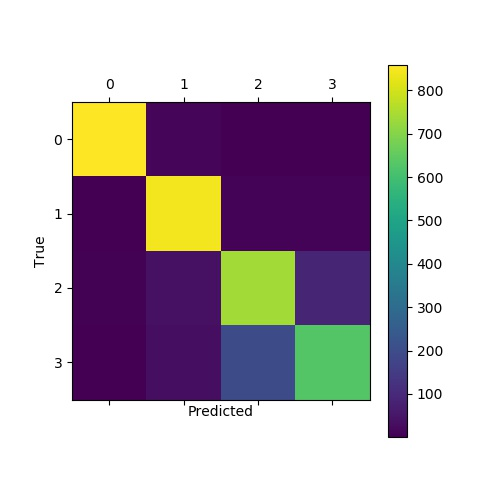
\includegraphics [scale=1.2] {confusion.jpg}
	\captionof{figure}{Results obtained shown with a Heat Map}
	\label{fig:confusion}
\end{figure}


\section{Results of Second Experiment}
The second method which involved using the pre-trained ImageNet model and retraining it with our dataset executed with just 200 epochs got a accuracy of 97\% with a cross entropy of 0.04. For retraining, 60\% of the whole dataset was training, 20\% for validation and 20\% was for testing. Table~\ref{table:confus}
shows the confusion matrix generated with the various score obtained after testing our model on 3485 random samples.
\begin{table}[!htbp]
	\centering \def\arraystretch{1.5} \small
	\begin{adjustbox}{max width=1.1\textwidth,center}
		
	\begin{tabular}{p{2cm}|p{2cm}|p{2cm}|p{2cm}|p{2cm}|p{2cm}|}
		
	\multicolumn{6}{c} {\textbf{Predicted}} \\ \cline{2-6}
			
       \multirow{6}{*} {\rotatebox{90}{\textbf{Truth}}} 
          
           &  & Bar chart & Box chart & Line chart & Scatter plot \\ \cline{2-6}	

			& Bar chart  &  850 \cellcolor[gray]{.8} & 12  & 2 & 2 \\  \cline{2-6}	 
			
			& Box 	plot & 19  &  822 \cellcolor[gray]{.8}& 5 & 20 \\ \cline{2-6}	   
			
			& Line Chart & 1 & 10 & 854 \cellcolor[gray]{.8} & 24 \\ 
			\cline{2-6}
			
			& Scatter plot & 1 & 1 & 7 & 855\cellcolor[gray]{.8} \\ \cline{2-6}
		
		\end{tabular}
		
	\end{adjustbox}
	\caption {Table showing confusion metrics generated with results obtained from the test data}
	\label{table:confus}	
\end{table}

From the confusion matrix, we observe that box plots were the least classified correctly with most of the predictions on box plots being misclassified as Scatter plots and Bar charts. Another interesting observation is that most of the misclassified sample of Bar charts were classified as Box plots. 

\section{Discussion}
Our results show that the AlexNet modified architecture of the CovNet used for the training and testing of our model works well, this is based on the good results gained in the first experiment, also the idea that we can transfer the knowledge learned from training a model on a huge dataset of a somewhat similar problem to our problem can improve our results stands to be true based on our accuracy moving from 89\% to 97\% when we retrained the ImageNet model with our chart dataset. I believe the results of this thesis was successful despite the difficulty of the task, from the results shown on the confusion matrix which led to us studying the misclassified samples we realized that in the first experiment 235 scatter plots were misclassified as line charts, the reason for this is that we had created quiet a number of line charts which had a regression line and these had a striking resemblance to a type of line chart with markers and a line showing the relationship between these markers. Also there were some scatter plots which were positive and negatively correlated with all markers appearing in a straight line and this could have been as well considered as a line chart by our classifier. Figure~\ref{fig:miss} shows sample scatter plots which resemble line charts. The class with the second most misclassified samples was unsurprisingly line charts being classified as scatter plots. As discussed previous some variants of line charts are very much like scatter plots and this explains the high number of misclassified line chart instances. There also quiet a number of box plots misclassified as line charts this can be attributed to the fact that box plots are made of lines and markers (outliers) which resemble a type of line chart with markers and a line connecting these markers. A number of box plots were misclassified as bar charts because box plots and bar charts are somehow similar in their appearance.
Figure~\ref{fig:missy} shows 9 randomly chosen misclassified charts after our model was tested.

\begin{figure}[!htb]
	\begin{subfigure}{.6\textwidth}
		\centering
		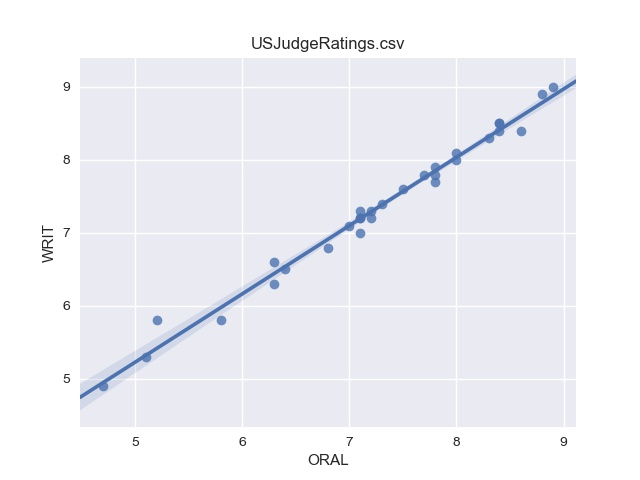
\includegraphics[width=.8\linewidth]{mis3.jpg}
		\caption{scatter plot}
		\label{fig:mis1}
	\end{subfigure}%
	\begin{subfigure}{.5\textwidth}
		\centering
		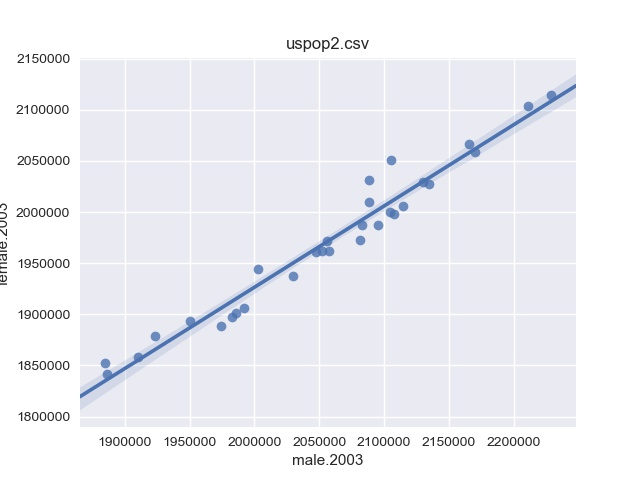
\includegraphics[width=1.0\linewidth]{mis2.jpg}
		\caption{scatter plot}
		\label{fig:mis2}
	\end{subfigure}
	\caption{Sample scatter plots with a best fit line created in python with the Plotly library}
	\label{fig:miss}
\end{figure}

\begin{figure}[!htbp]
	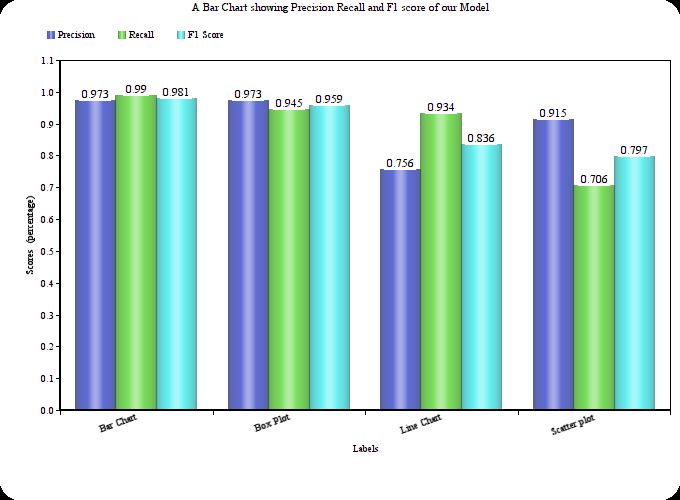
\includegraphics [scale=0.78] {scores.png}
	\captionof{figure}{A bar chart showing the precision recall and F1 scoreof our experiment}
	\label{fig:missy}
\end{figure}

The hypothesis we came up with from the results in the first experiment are affirmed from the results achieved in the second experiment. In the second experiment results show that line charts were mostly misclassified as scatter plots as in the case of the first experiment. 

The results from the second experiment that were surprisingly different from the first experiment  were the high number of box plots misclassified as scatter plots. We attribute this to the fact that box plots contain outliers (markers) which scatter plots also contain therefore the issue. Figure \ref{fig:missrand} shows a few samples and what they were misclassified as in the second experiment. 

\begin{figure}[!htb]
	\begin{subfigure}{.6\textwidth}
		\centering
		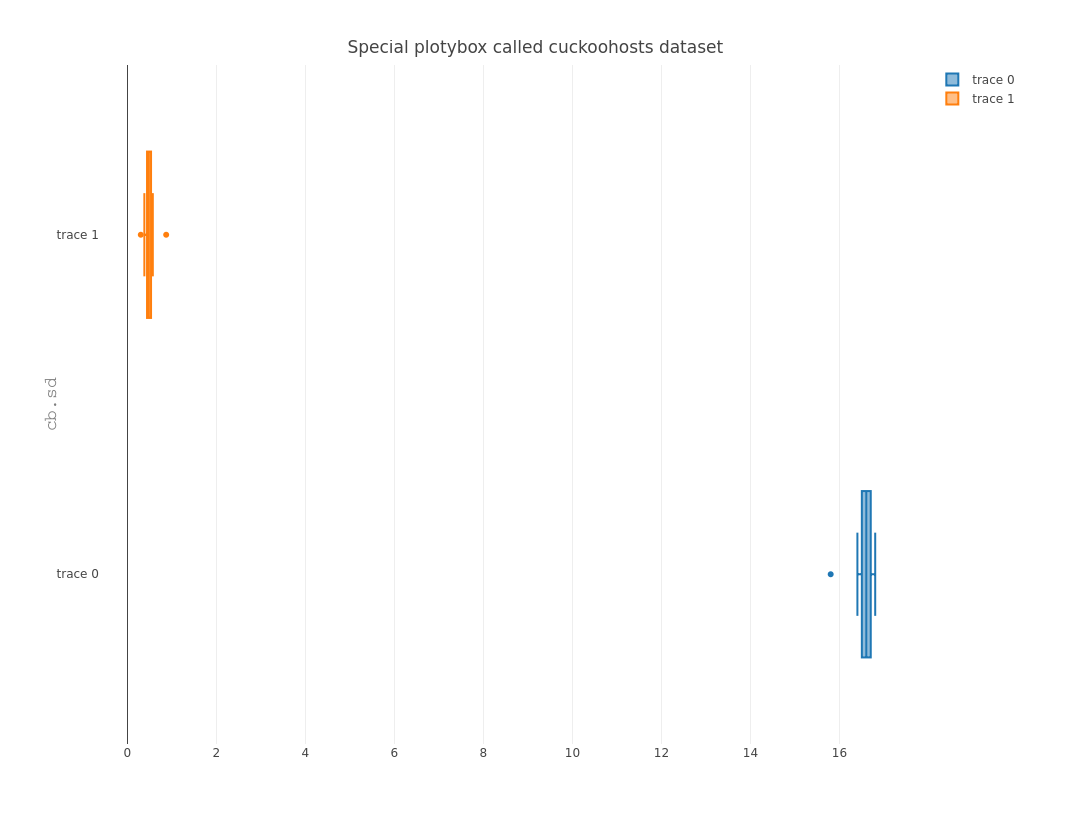
\includegraphics[width=.8\linewidth]{missyscatter.png}
		\caption{Box plot misclassified as scatter plot}
		\label{fig:mis1}
	\end{subfigure}%
	\begin{subfigure}{.5\textwidth}
		\centering
		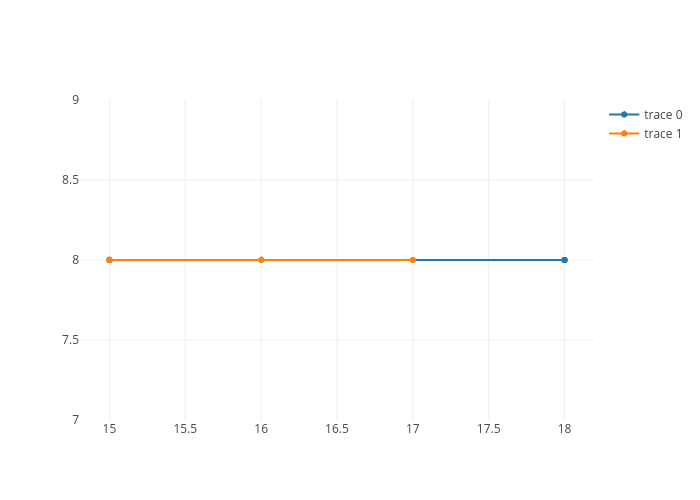
\includegraphics[width=1.0\linewidth]{missyscatter2.png}
		\caption{Line chart misclassified as scatter plot}
		\label{fig:mis2}
	\end{subfigure}
	\caption{Sample plots misclassified in the second experiment}
	\label{fig:missrand}
\end{figure}



\begin{figure}[!htb]
	\begin{subfigure}{.6\textwidth}
		\centering
		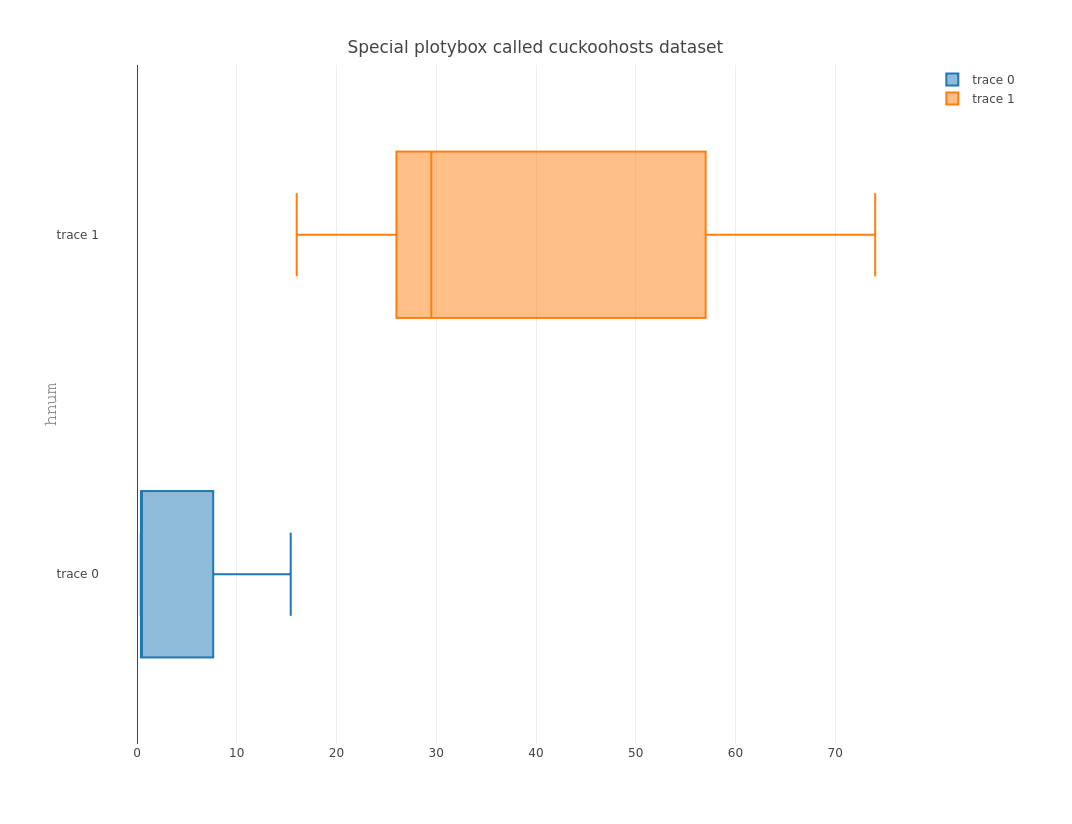
\includegraphics[width=.8\linewidth]{missybar.png}
		\caption{Box plot misclassified as bar chart}
		\label{fig:mis1}
	\end{subfigure}%
	\begin{subfigure}{.5\textwidth}
		\centering
		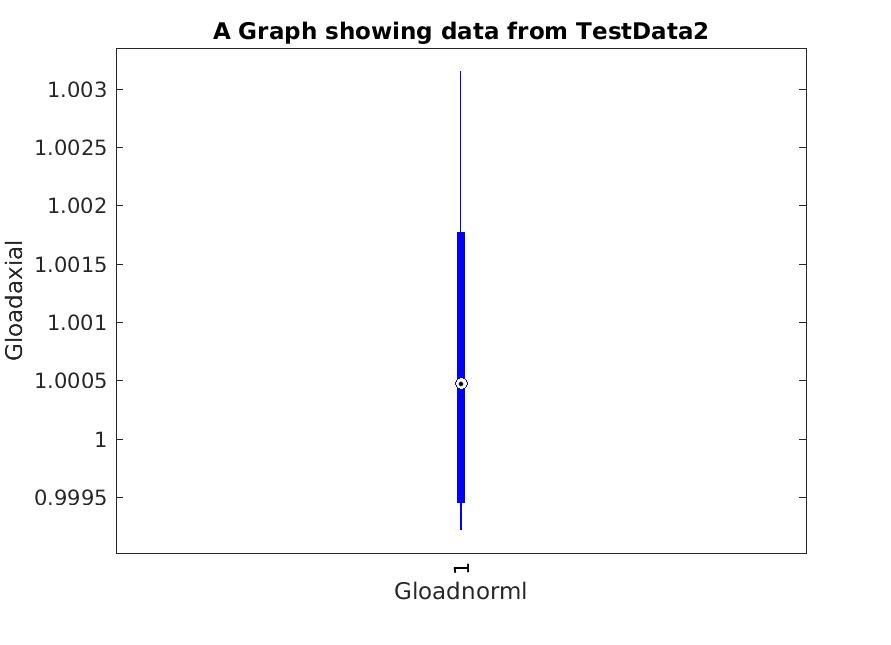
\includegraphics[width=1.0\linewidth]{missyline.jpg}
		\caption{Box plot misclassified as a Line chart}
		\label{fig:mis2}
	\end{subfigure}
	\caption{Sample plots misclassified in the second experiment}
	\label{fig:missrand2}
\end{figure}

\chapter{Summary}

\bibliographystyle{unsrt}
\bibliography{sample}

\end{document}=====